\documentclass[a4paper, twoside]{report}
\usepackage[margin=0.5in]{geometry}
\usepackage{amsmath}
\usepackage{amsfonts}
\usepackage{amssymb}
\usepackage{amsthm}
\usepackage{graphicx}
\usepackage{physics}
\usepackage{tikz}
\usepackage{mathrsfs}
\usepackage{pgfplots}
\usepgfplotslibrary{polar}
\usepgfplotslibrary{fillbetween}
\pgfplotsset{compat=1.18}
\usetikzlibrary{arrows,patterns, backgrounds, calc,fadings,shadows.blur, shapes}
\theoremstyle{plain}
\usepackage[most]{tcolorbox}
\usepackage{physunits}
\usepackage{float}
\usepackage[stable]{footmisc}
\usepackage{xcolor}
\usepackage{wrapfig}
\usepackage{microtype}
\usepackage{thmtools}
\usepackage[framemethod=TikZ]{mdframed}
\usepackage{steinmetz}
\usepackage{adjustbox}
\usepackage{listings}
\usepackage[version=4]{mhchem}
\newcommand{\floor}[1]{\lfloor #1 \rfloor}
\newcommand*{\Perm}[2]{{}^{#1}\!P_{#2}}%
\newcommand*{\Comb}[2]{{}^{#1}C_{#2}}%
\mdfsetup{skipabove=1em,skipbelow=0em}
\tcbuselibrary{xparse}
\usepackage[font=small,labelfont=bf,margin=\parindent,tableposition=top]{caption}
\newenvironment{solution}
{\renewcommand\qedsymbol{$\blacksquare$}\begin{proof}[Solution]}
	{\end{proof}}


\declaretheoremstyle[
headfont=\bfseries\sffamily\color{blue!70!black}, bodyfont=\normalfont,
mdframed={
	linewidth=2pt,
	rightline=false, topline=false, bottomline=false,
	linecolor=blue, backgroundcolor=blue!5,
}
]{thmbluebox}
\declaretheorem[style=thmbluebox, numbered=no, name=Example]{eg}


\declaretheoremstyle[
headfont=\bfseries\sffamily\color{blue!70!black}, bodyfont=\normalfont,
numbered=no,
mdframed={
	linewidth=2pt,
	rightline=false, topline=false, bottomline=false,
	linecolor=blue, backgroundcolor=blue!1,
},
]{thmexplanationbox}
\declaretheorem[style=thmexplanationbox, name=Solution]{tmpexplanation}
\newenvironment{explanation}[1][]{\vspace{-10pt}\begin{tmpexplanation}}{\end{tmpexplanation}}


\declaretheoremstyle[
headfont=\bfseries\sffamily\color{red!70!black}, bodyfont=\normalfont,
mdframed={
	linewidth=2pt,
	rightline=false, topline=false, bottomline=false,
	linecolor=red, backgroundcolor=red!5,
}
]{thmredbox}
\declaretheorem[style=thmredbox, name=Theorem]{theorem}

\declaretheoremstyle[
headfont=\bfseries\sffamily\color{red!70!black}, bodyfont=\normalfont,
numbered=no,
mdframed={
	linewidth=2pt,
	rightline=false, topline=false, bottomline=false,
	linecolor=red, backgroundcolor=red!2,
},
qed=\qedsymbol
]{thmproofbox}
\declaretheorem[style=thmproofbox, name=Proof]{replacementproof}
\renewenvironment{proof}[1][\proofname]{\vspace{-10pt}\begin{replacementproof}}{\end{replacementproof}}

\declaretheoremstyle[
headfont=\bfseries\sffamily\color{brown!70!black}, bodyfont=\normalfont,
mdframed={
	linewidth=2pt,
	rightline=false, topline=false, bottomline=false,
	linecolor=brown, backgroundcolor=brown!5,
}
]{thmbrownbox}
\declaretheorem[style=thmbrownbox, numbered=no, name=Question]{asign}

\declaretheoremstyle[
headfont=\bfseries\sffamily\color{brown!70!black}, bodyfont=\normalfont,
numbered=no,
mdframed={
	linewidth=2pt,
	rightline=false, topline=false, bottomline=false,
	linecolor=brown, backgroundcolor=brown!1,
},
]{thmansbox}
\declaretheorem[style=thmansbox, name=Answer]{thmbrown}
\newenvironment{anse}[1][]{\vspace{-10pt}\begin{thmbrown}}{\end{thmbrown}}

\tikzset {_uty0p60aj/.code = {\pgfsetadditionalshadetransform{ \pgftransformshift{\pgfpoint{0 bp } { 0 bp }  }  \pgftransformrotate{-270 }  \pgftransformscale{2 }  }}}
\pgfdeclarehorizontalshading{_zo7gli6ny}{150bp}{rgb(0bp)=(0.6,0.85,1);
rgb(53.66071428571429bp)=(0.6,0.85,1);
rgb(61.60714285714286bp)=(0,0.5,0.5);
rgb(100bp)=(0,0.5,0.5)}
\tikzset{every picture/.style={line width=0.75pt}} %set default line width to 0.75pt 

\usepackage[hidelinks]{hyperref}

\begin{document}

	\begin{titlepage}
		\begin{center}
			\Huge{Mathematics-1 (FCMT001)}\\
			Srijan Mahajan (2023UCM2326)\\
			Prof. Sarika
		\end{center}
	\end{titlepage}
	\tableofcontents
	\newpage

	\chapter{Functions of Single Variable}
	Some common sets are,
	\begin{itemize}
		\item $\mathbb{R}$ It is the set of all real numbers
		\item $\mathbb{N}$ It is the set of all natural numbers
		\item $\mathbb{Z}$ It is the set of all integers
		\item $\mathbb{Q}$ It is the set of all rationals
		\item $\mathbb{Q}^\complement$ It is the set of all irrationals
	\end{itemize}
	Also, $\mathbb{R}=\mathbb{Q} \cup \mathbb{Q}^\complement$.
	\begin{theorem}[Uncountable $\mathbb{Q}^\complement$]
		The set of all irrationals is uncountable.
	\end{theorem}
	\begin{proof}
		We know, $\mathbb{R}$ is uncountable and $\mathbb{Q}$ is uncountable, since,
		\[\mathbb{R}=\mathbb{Q} \cup \mathbb{Q}^\complement\]
		$\mathbb{Q}^\complement$ must be uncountable.
	\end{proof}
	\section{Ranges}
	\subsection{Maximum and Minimum}
	The maxima is the highest element in the set and similarly, minima is the lowest element in the set.\footnote{Maximum and minimum are unique for a set, i.e. there exists only one for a given set.}
	\begin{eg}[Max and min not enough]
		Find the maximum and minimum of
		\[S=\{\frac{1}{n} | n \in \mathbb{N}\}\]
	\end{eg}
	\begin{explanation}
		Here, the set can be represented as,
		\[S\in \left( 0, 1 \right]\]
		Here, the maximum value is clearly 1, however, the minimum vale of the expression can't be defined\footnote{Since 0 is not in the set and also, 0 is never actually obtained but only close to.}.
	\end{explanation}
	\subsection{Infimum and Supremum}
	The infimum of a set is its greatest lower bound and supremum is the lowest upper bound. These are generalizations of maximum and minimum.
	\begin{eg}
		Find the infimum and supremum of
		\[S=\{\frac{1}{n} | n \in \mathbb{N}\}\]
	\end{eg} 
	\begin{explanation}
		Similarly,
		\[S=\left( 0, 1 \right] \]
		Thus, the infimum is 0 and supremum is 1.
	\end{explanation}
	\begin{eg}[Not always in set]
		Find the infimum and supremum of
		\[S=\{ x^2\leq 2 | x\in \mathbb{Q}^+ \}\]
	\end{eg}
	\begin{explanation}
		\[x\in (0, \sqrt{2} ]\]
		Here, $x$ is defined in the natural numbers but the supremum is not in $\mathbb{Q}^+$. Thus, infimum and supremum are not always a part of the set.
	\end{explanation}
	\begin{eg}
		Find the infimum and supremum of
		\[S=\{1+\frac{(-1)^n}{n} | n\in \mathbb{N}\}\]
	\end{eg}
	\begin{explanation}
		The next few digits are, $0, \frac{3}{2}, \frac{2}{3}, \frac{5}{4}, \cdots$. Hence, infimum is 0 and supremum is $\frac{3}{2}$.
	\end{explanation}
	\section{Bounded Set}
	A set is said to be bounded if it has both upper and lower bounds. E.g. $(0, \infty)$ has a lower bound but no upper bound.
	\begin{eg}[Finite]
		Is the given set finite/infinite, bounded/unbounded and find infimum and supremum (if exists),
		\[S= \{ \sin(\frac{n\pi}{2}) | n\in \mathbb{Z} \}\]
	\end{eg}
	\begin{explanation}
		The range of the set is,
		\[ran(S)=\{-1,0,1\}\]
		Since the cardinality is finite, the set $S$ is said to be finite, and bounded. Clearly, the infimum is $-1$ and the supremum is $1$.
	\end{explanation}
	\section{Limits}
	\begin{theorem}[Continuity]
		A function $f: S \subseteq \mathbb{R} \to \mathbb{R}$ is continuous at $x=a$ if,
		\[\lim\limits_{x\to a^-}f(x)=\lim\limits_{x\to a^+}f(x)=\lim\limits_{x\to a}f(x)=f(a)\]
	\end{theorem}
	\begin{theorem}[Limit Exists]
		Let $S\subset \mathbb{R}$ and $f:S\to \mathbb{R}$, we can say $\lim\limits_{x\to a}f(x)=L$ if,
		\[\lim\limits_{x\to a^-}f(x)=\lim\limits_{x\to a^+}f(x)=L\]
	\end{theorem}
	We can say that the limit exists at some point when the function approaches the value from both sides (left and right hand limit), however, this works only in the case of $\mathbb{R}$. It fails in $\mathbb{R}^n$, as the point can be achieved from infinitely many directions (disc/sphere).
	\begin{theorem}[$\epsilon-\delta$ definition of a limit]
		Let $f(x)$ be a real valued function defined on an open interval around $a$.
		\[\lim\limits_{x\to a}f(x)=L\text{ , if } \forall \epsilon>0, \exists \delta>0 (\forall x>0, 0<|x-a|<\delta \implies |f(x)-L|<\epsilon)\]
			\begin{figure}[H]
				\centering			
				\tikzset{every picture/.style={line width=0.75pt}} %set default line width to 0.75pt        			
				\begin{tikzpicture}[x=0.75pt,y=0.75pt,yscale=-1,xscale=1]
					%uncomment if require: \path (0,329); %set diagram left start at 0, and has height of 329			
					%Straight Lines [id:da39637912070401926] 
					\draw    (90,277.11) -- (90,22) ;
					\draw [shift={(90,20)}, rotate = 90] [color={rgb, 255:red, 0; green, 0; blue, 0 }  ][line width=0.75]    (10.93,-3.29) .. controls (6.95,-1.4) and (3.31,-0.3) .. (0,0) .. controls (3.31,0.3) and (6.95,1.4) .. (10.93,3.29)   ;
					%Straight Lines [id:da014662667668136953] 
					\draw    (90,277.11) -- (418,277) ;
					\draw [shift={(420,277)}, rotate = 179.98] [color={rgb, 255:red, 0; green, 0; blue, 0 }  ][line width=0.75]    (10.93,-3.29) .. controls (6.95,-1.4) and (3.31,-0.3) .. (0,0) .. controls (3.31,0.3) and (6.95,1.4) .. (10.93,3.29)   ;
					%Curve Lines [id:da3684607671706839] 
					\draw    (130,180) .. controls (317,235) and (184,41) .. (400,60) ;
					%Straight Lines [id:da8088388105686377] 
					\draw  [dash pattern={on 0.84pt off 2.51pt}]  (253,136) -- (255,277.06) ;
					%Straight Lines [id:da3809187691914382] 
					\draw  [dash pattern={on 0.84pt off 2.51pt}]  (357,58.94) -- (359,277) ;
					%Straight Lines [id:da8808960388225944] 
					\draw  [dash pattern={on 0.84pt off 2.51pt}]  (90,137) -- (253,136) ;
					%Straight Lines [id:da32340812817097375] 
					\draw  [dash pattern={on 0.84pt off 2.51pt}]  (91,59.94) -- (357,58.94) ;				
					% Text Node
					\draw (437,272.4) node [anchor=north west][inner sep=0.75pt]    {$x$};
					% Text Node
					\draw (241,282.4) node [anchor=north west][inner sep=0.75pt]    {$a-\delta $};
					% Text Node
					\draw (341,282.4) node [anchor=north west][inner sep=0.75pt]    {$a-\delta $};
					% Text Node
					\draw (301,282.4) node [anchor=north west][inner sep=0.75pt]    {$a$};
					% Text Node
					\draw (298,92.4) node [anchor=north west][inner sep=0.75pt]    {$f( x)$};
					% Text Node
					\draw (51,129.4) node [anchor=north west][inner sep=0.75pt]    {$L-\epsilon $};
					% Text Node
					\draw (51,52.4) node [anchor=north west][inner sep=0.75pt]    {$L+\epsilon $};
					% Text Node
					\draw (61,92.4) node [anchor=north west][inner sep=0.75pt]    {$L$};
				\end{tikzpicture}
			\end{figure}
	\end{theorem}
	Clearly, if $f(a)=L$, then $f$ is continuous.
	\subsection{Sequence Definition of a Limit}
	A sequence $\{x_n\}$ is a $f:\mathbb{N}\to \mathbb{R}$ such that $f(n)=x_n$.\\
	If $x_n \to a \, (a\in \mathbb{R})$, then the sequence is said to be convergent, else convergent/oscillating.
	\begin{theorem}[Non-existing Limit]
		$\lim\limits_{x\to a}f(x)$ doesn't exist iff 
		\[\begin{split}
			\lim\limits_{n\to \infty} f(x_n)&=L_1\\
			\lim\limits_{n\to \infty} f(y_n)&=L_2\\
		\end{split}\]
		where $L_1\neq L_2$ and $x_n\to a \land y_n \to a$ as $n\to \infty$.
	\end{theorem}
	To prove that a limit exists, it must satisfy $\lim\limits_{n\to\infty}f(x_n)=L$ for all sequences $x_n$.
	\begin{eg}
		Find the limit
		\[\lim\limits_{x\to 0} \sin(\frac{1}{x})\]
	\end{eg}
	For these, we need to work backwards, first we take two values that the function can take (here 0 and 1), then find two sequences that converge to the same but give the respective values.
	\begin{explanation}
		Consider,
		\[x_n=\frac{1}{2n\pi} \, \land \, y_n=\frac{1}{2n\pi+\frac{\pi}{2}}\]
		Clearly,
		\[f(x_n)=0\land f(y_n)=1\]
		But $\lim\limits_{n\to\infty}x_n=\lim\limits_{n\to\infty}y_n=0$. Thus, the limit doesn't exist.
	\end{explanation}
	\begin{eg}[Someone]
		Show that the limit $\lim\limits_{x\to 0} \frac{|x|}{x}$ doesn't exist.
	\end{eg}
	\begin{explanation}
		Consider the sequences,
	\[	\begin{split}
			x_n=\frac{1}{n} \land y_n=-\frac{1}{n}
		\end{split}\]
		Clearly, $\lim\limits_{n\to \infty}x_n=\lim\limits_{n\to \infty}y_n=0$
		Also,
		\[\lim\limits_{n\to \infty} \frac{|\frac{1}{n}|}{\frac{1}{n}}=1 \land \lim\limits_{n\to \infty} \frac{|-\frac{1}{n}|}{-\frac{1}{n}}=-1 \]
		Thus, the limit doesn't exist.
	\end{explanation}
	\begin{eg}
		Show that $f$ is continuous at $x=\frac{1}{2}$ and discontinuous everywhere else, where $f$ is,
		\[f(x)=\begin{cases}
			x &, x\in \mathbb{Q}\\
			\frac{1}{2} &, x\notin \mathbb{Q}
		\end{cases}\]
	\end{eg}
	\begin{explanation}
		Consider the Left Hand Limit,
		\[\lim\limits_{x\to \frac{1}{2}^-}f(x)=\lim\limits_{h\to 0}f(\frac{1}{2}-h)=\begin{cases}
		\lim\limits_{h\to0}\frac{1}{2}-h &, x\in \mathbb{Q}\\
		\lim\limits_{h\to0}\frac{1}{2} &, x\notin \mathbb{Q}
		\end{cases}=\frac{1}{2}\]
		Similarly, Right Hand Limit is $\frac{1}{2}$, thus the function is continuous at $x=\frac{1}{2}$.\\
		Consider any point $x=a\in \mathbb{R}-\{\frac{1}{2}\}$,
		\[\lim\limits_{x\to a^-}f(x)=\begin{cases}
		\lim\limits_{h\to 0} a-h &, a-h\in \mathbb{Q}\\
		\lim\limits_{h\to 0} \frac{1}{2}&, a-h\notin \mathbb{Q}
		\end{cases}\]
		Thus the limit doesn't exist.
	\end{explanation}
	\begin{theorem}[Intermediate Value Theorem: A Special Case]
		Consider a continuous function $f$ on $[a,b]$ such that $f(a)f(b)<0$, then, $\exists c\in (a,b)$ such that $f(c)=0$.
	\end{theorem}
	\section{Differentiability}
	\begin{theorem}[A differentiable function]
		A function $f: S\neq \phi \subseteq \mathbb{R}\to \mathbb{R}$ is called differentiable at $x=a$ iff the following limit exists,
		\[\lim\limits_{x\to a}\frac{f(x)-f(a)}{x-a}\]
		If the limit does exist,
		\[\lim\limits_{x\to a}\frac{f(x)-f(a)}{x-a}=f'(a)\]
	\end{theorem}
	\begin{eg}
		Show $f$ is continuous at $x=0$,
		\[f(x)=\begin{cases}
			x^2\sin(\frac{1}{x}) &, x\neq 0\\
			0 &, x=0
		\end{cases}\]
	\end{eg}
	\begin{explanation}
		Suppose $\epsilon>0$. Now choose $\delta=\sqrt{\epsilon}$,\\
		Let $|x-0|<\delta$.
		Check,
		\[\begin{split}
			&|x^2\sin(\frac{1}{x})\\
			\leq & |x|^2\\
			\leq &\delta^2\\
			=& \epsilon
		\end{split}\]
		Thus, $|x^2\sin(\frac{1}{x})|<\epsilon$, so, $f$ is continuous at $x=0$.
	\end{explanation}
	\begin{theorem}[Rolle's Theorem]
		Let $f:[a,b]\to\mathbb{R}$ be a continuous function on its domain and be differentiable on $(a,b)$, such that $f(a)=f(b)$, then $\exists c\in(a,b)$ such that, $f'(c)=0$.
	\end{theorem}
	\begin{theorem}[Lagrange Mean Value Theorem]
		Let $f:[a,b]\to\mathbb{R}$ be a continuous function on its domain and be differentiable on $(a,b)$, then $\exists c\in(a,b)$ such that, $f'(c)=\frac{f(b)-f(a)}{b-a}$.
	\end{theorem}
	\begin{proof}
		We can prove this using Rolle's Theorem. It is an extension of Rolle's Theorem.
	\end{proof}
	\section{Tutorial-1 (19.08.2023)}
\subsection{Examine the limit and continuity of the following functions}
\begin{asign}
	\[f(x)=\lim\limits_{n\to\infty}\frac{e^x-x^n\sin x}{1+x^n} \, , 0\leq x\leq\frac{\pi}{2}\, \text{at} \, x=1\]
\end{asign}
\begin{anse}
	We can split the function at $x=1$,
	\[\begin{split}
		f(x)&=\begin{cases}
			\lim\limits_{n\to\infty}\frac{e^x-x^n\sin x}{1+x^n} &, 0\leq x < 1\\
			\lim\limits_{n\to\infty}\frac{e^x-x^n\sin x}{1+x^n} &, x=1\\
			\lim\limits_{n\to\infty}\frac{e^x-x^n\sin x}{1+x^n} &, 1<x\leq \frac{\pi}{2}
		\end{cases}\\
		&=\begin{cases}
			e^x &,  0\leq x < 1\\
			\frac{e-\sin 1}{2} &, x=1\\
			-\sin x &, 1<x\leq \frac{\pi}{2}
		\end{cases}
	\end{split}\]
	Thus, clearly, $f$ is discontinuous at $x=1$.
\end{anse}
\begin{asign}
	\[f(x)=\begin{cases}
		x^2\cos(\frac{1}{x}) &, x\neq0\\
		0 &, x=0
	\end{cases} \, \text{at} \, x=0 \]
\end{asign}
\begin{anse}
	First we calculate the limit
	\[\begin{split}
		L&=\lim\limits_{x\to 0}x^2\cos(\frac{1}{x})\\
		&=0
	\end{split}\]
	Here, $\lim\limits_{x\to0}f(x)=f(0)$, thus the function is continuous.
\end{anse}
\begin{asign}
	\[f(x)=\begin{cases}
		\sin(\frac{1}{x-a}) &, x\neq a\\
		0 &, x=a
	\end{cases} \, \text{at} \, x=a\]
\end{asign}
\begin{anse}
	Consider,
	\[
	\begin{split}
		&x_n=a+\frac{1}{2n\pi}\\
		&\lim\limits_{n\to \infty}x_n=a
	\end{split}
	\quad  \quad
	\begin{split}
		&y_n=a+\frac{1}{2n\pi+\frac{\pi}{2}}\\
		&\lim\limits_{n\to\infty}y_n=a
	\end{split}
	\]
	Also,
	\[f(x_n)=0\,\land\, f(y_n)=1\]
	Thus, by Sequence Criteria, $f$ is discontinuous at $x=a$.
\end{anse}
\begin{asign}
	\[f(x)=\begin{cases}
		\frac{e^{\frac{1}{x}}-e^{-\frac{1}{x}}}{e^{\frac{1}{x}}+e^{-\frac{1}{x}}} &, x\neq 0\\
		0 &, x=0
	\end{cases} \, \text{at}\, x=0\]
\end{asign}
\begin{anse}
	Consider the Left Hand Limit,
	\[\lim\limits_{x\to0^-}\frac{e^{\frac{1}{x}}-e^{-\frac{1}{x}}}{e^{\frac{1}{x}}+e^{-\frac{1}{x}}}=\lim\limits_{x\to0^-}\frac{e^{\frac{2}{x}}-1}{e^{\frac{2}{x}}+1}=-1\]
	As $\lim\limits_{x\to0^-}f(x)\neq f(0)$ the function is discontinuous at $x=0$.
\end{anse}
\begin{asign}
	\[f(x)=\begin{cases}
		\frac{\sin[2](ax)}{x^2} &, x\neq 0\\
		0, &, x=0
	\end{cases} \, a\in \mathbb{R}\]
\end{asign}
\begin{anse}
	\[\lim\limits_{x\to 0}f(x)=\lim\limits_{x\to0}\frac{\sin[2](ax)}{(ax)^2}\cdot a^2=a^2\]
	Thus, the function is discontinuous for all $a\in\mathbb{R}-\{0\}$, i.e. it is continuous at $a=0$.
\end{anse}
\begin{asign}
	\[f(x)=\begin{cases}
		\frac{1-\cos x}{x^2} &, x\neq0\\
		\frac{1}{2} &, x=0
	\end{cases} \, \text{at} \, x=0\]
\end{asign}
\begin{anse}
	\[\lim\limits_{x\to0}f(x)=\lim\limits_{x\to0} \frac{1-\cos x}{x^2}=\frac{1}{2}\lim\limits_{x\to0}\frac{\sin^2(\frac{x}{2})}{(\frac{x}{2})^2}=\frac{1}{2}\]
	Since $\lim\limits_{x\to0}f(x)=f(0)$, the function is continuous at $x=0$.
\end{anse}
\begin{asign}
	\[f(x)=\begin{cases}
		\frac{(x-1)-|x-1|}{x-1} &, x\neq 1\\
		2 &, x=1
	\end{cases} \, \text{at}\, x=1\]
\end{asign}
\begin{anse}
	Consider the Right Hand Limit,
	\[\lim\limits_{x\to 1^+}\frac{(x-1)-|x-1|}{x-1} =\lim\limits_{x\to1^+}\frac{(x-1)-(x-1)}{x-1}=0\]
	As $\lim\limits_{x\to1^+}f(x)\neq f(1)$, the function is discontinuous at $x=1$.
\end{anse}
\subsection{Are the following functions continuous and differentiable}
\begin{asign}
	\[f(x)=\begin{cases}
		2+x &, x\geq0\\
		2-x &, x\leq0
	\end{cases} \, \text{at} \, x=0\]
\end{asign}
\begin{anse}
	\[\lim\limits_{x\to0^-}f(x)=2 \land \lim\limits_{x\to 0^+}f(x)=2\land f(0)=2\]
	Thus, the function is continuous at $x=2$.
	For differentiability,
	\[\lim\limits_{x\to 0^-}\frac{f(x)-f(0)}{x}=\lim\limits_{x\to0^-}\frac{2+x-2}{x}=1 \land \lim\limits_{x\to 0^+}\frac{f(x)-f(0)}{x}=\lim\limits_{x\to0^+}\frac{2-x-2}{x}=-1\]
	Thus, the function is not differentiable at $x=0$.
\end{anse}
\begin{asign}
	\[f(x)=\begin{cases}
		x^2-1 &, x\geq 1\\
		1-x &, x\leq1 
	\end{cases}\,\text{at}\, x=1\]
\end{asign}
\begin{anse}
	\[\lim\limits_{x\to1^-}f(x)=\lim\limits_{x\to1^+}f(x)=f(1)=0\]
	Thus, the function is continuous at $x=1$. For differentiability,
	\[\lim\limits_{x\to1^-}\frac{f(x)-f(1)}{x-1}=\lim\limits_{x\to 1^-}\frac{x^2-1-0}{x-1}=2 \land \lim\limits_{x\to1^+}\frac{f(x)-f(1)}{x-1}=\lim\limits_{x\to 1^+}\frac{1-x-0}{x-1}=-1\]
	Thus, the function is not differentiable at $x=1$.
\end{anse}
\begin{asign}
	\[f(x)=\begin{cases}
		x\frac{e^{\frac{1}{x}}-e^{-\frac{1}{x}}}{e^{\frac{1}{x}}+e^{-\frac{1}{x}}} &, x\neq 0\\
		0 &, x=0
	\end{cases}\,\text{at}\,x=0\]
\end{asign}
\begin{anse}
	Clearly, due to multiplication of $x$, the function is continuous at $x=0$. For differentiability,
	\[\lim\limits_{x\to0^-}\frac{f(x)-f(0)}{x}=-1 \land \lim\limits_{x\to0^+}\frac{f(x)-f(0)}{x}=1 \]
	Thus, the function is not differentiable at $x=0$.
\end{anse}
\begin{asign}
	\[f(x)=\begin{cases}
		x\tan^{-1}(\frac{1}{x}) &, x\neq0\\
		0 &, x=0
	\end{cases} \,\text{at}\,x=0\]
\end{asign}
\begin{anse}
	We know,
	\[\begin{split}
		-\frac{\pi}{2} < &\tan^{-1}(\frac{1}{x}) <\frac{\pi}{2}\\
		\implies -\frac{\pi}{2}x < &x\tan^{-1}(\frac{1}{x}) <\frac{\pi}{2}x\\
		\therefore 0<&\lim\limits_{x\to0}x\tan^{-1}(\frac{1}{x}) <0
	\end{split}\]
	Thus, $\lim\limits_{x\to0}x\tan^{-1}(\frac{1}{x})=0$. Hence, the function is continuous at $x=0$. For differentiability,
	\[\lim\limits_{x\to0}\frac{f(x)-f(0)}{x}=\lim\limits_{x\to0}\tan^{-1}(\frac{1}{x}) \, \text{Does not exist} \]
	Thus, the function is not differentiable at $x=0$.
\end{anse}
\begin{asign}
	\[f(x)=\begin{cases}
		2x &, x\in\mathbb{Q}\\
		-2x &, x\notin\mathbb{Q}
	\end{cases}\,\text{at}\, x=0\]
\end{asign}
\begin{anse}
	\[\lim\limits_{x\to0^-}f(x)=\lim\limits_{h\to0^-}f(h)=\begin{cases}
		2h &, h\in\mathbb{Q}\\
		-2h &, h\notin\mathbb{Q}
	\end{cases}=0\]
	Similarly, for the Right Hand Limit. Thus, the function is continuous at $x=0$. For differentiability,
	\[\lim\limits_{x\to0}\frac{f(x)-f(0)}{x}=\lim\limits_{x\to 0}\frac{f(x)}{x}=\begin{cases}
		2 &, x\in\mathbb{Q}\\
		-2 &, x\notin\mathbb{Q}
	\end{cases}\]
	Thus, the function is not differentiable at $x=0$.
\end{anse}
\begin{asign}
	\[f(x)=\begin{cases}
		x^2 &, x\in\mathbb{Q}\\
		2x &, x\notin\mathbb{Q}
	\end{cases}\,\text{at}\, x=0\]
\end{asign}
\begin{anse}
	\[\lim\limits_{x\to0^-}f(x)=\lim\limits_{h\to0^-}f(h)=\begin{cases}
		h^2 &, h\in\mathbb{Q}\\
		2h &, h\notin\mathbb{Q}
	\end{cases}=0\]
	Similarly, for the Right Hand Limit. Thus, the function is continuous at $x=0$. For differentiability,
	\[\lim\limits_{x\to0}\frac{f(x)-f(0)}{x}=\lim\limits_{x\to 0}\frac{f(x)}{x}=\begin{cases}
		x &, x\in\mathbb{Q}\\
		2 &, x\notin\mathbb{Q}
	\end{cases}\]
	Thus, the function is not differentiable at $x=0$.
\end{anse}
\subsection{Question 3}
\begin{asign}
	Show that the function $f$ defined by  $f(x)=\begin{cases}
		x^2\cos(\frac{1}{x}) &, x\neq0\\
		0 &, x=0
	\end{cases}$ is continuous and differentiable at $x=0$ but its derivative is not.
\end{asign}

\begin{anse}
	We know,
	\[\begin{split}
		-1< &\cos(\frac{1}{x})< 1\\
		\implies -x^2 < & x^2\cos(\frac{1}{x})<x^2\\
		\therefore 0<& \lim\limits_{x\to 0}x^2\cos(\frac{1}{x})<0
	\end{split}\]
	Thus, $\lim\limits_{x\to0}x^2\cos(\frac{1}{x})=0$. Thus, $f$ is continuous at $x=0$. For differentiability,
	\[\lim\limits_{x\to0}\frac{f(x)-f(0)}{x}=\lim\limits_{x\to0}x\cos(\frac{1}{x})=0\]
	Thus, the function is differentiable at $x=0$. The derivative is,
	\[f'(x)=\begin{cases}
		2x\cos(\frac{1}{x})+\sin(\frac{1}{x}) &, x\neq0\\
		0 &, x=0
	\end{cases}\]
	Clearly, $\sin(\frac{1}{x})$ is discontinuous at $x=0$, thus, $f'(x)$ is discontinuous at $x=0$.
\end{anse}
\subsection{Question 4}
\begin{asign}
	Show that the function $f$ defined by  $f(x)=\begin{cases}
		x^p\cos(\frac{1}{x}) &, x\neq0\\
		0 &, x=0
	\end{cases}$ is continuous and differentiable at $x=0$ but its derivative is not.
\end{asign}
\begin{anse}
	We know,
	\[\begin{split}
		-x^p<&x^p\cos(\frac{1}{x}) < x^p
	\end{split}\]
	Thus, the limit exists only if $p>0$. Thus, $f$ is continuous for $p>0$.  For differentiability,
	\[\lim\limits_{x\to0} x^{p-1}\cos(\frac{1}{x})\]
	This limit exists only when $p>1$. Thus, $f$ is differentiable for $p>1$.
	\[f'(x)=\begin{cases}
		px^{p-1}\cos(\frac{1}{x})+x^{p-2}\sin(\frac{1}{x}) &, x\neq0\\
		0 &, x=0
	\end{cases}\]
	This is continuous for $p>2$. Thus $f'(x)$ is continuous for $p>2$.
\end{anse}
\subsection{Applications of IVT, Rolle's Theorem and MVT}
\subsubsection{Determine if the following equations admits solution in the interval mentioned}
\begin{asign}
	\[x^5-3x^2=-1\]
	in $[0,1]$
\end{asign}
\begin{anse}
	Let,
	\[f(x)=x^5-3x^2+1\implies f(0)=1\land f(1)=-1\]
	Since $f(0)f(1)<0$, by Intermediate Value Theorem, there is a solution in the interval.
\end{anse}
\begin{asign}
	\[\sin^2x-2\cos x=-1\]
	in $[0,\frac{\pi}{2}]$
\end{asign}
\begin{anse}
	Let,
	\[f(x)=\sin^2x-2\cos x+1 \implies f(0)=-1 \land f(\frac{\pi}{1})=2\]
	Since $f(0)f(\frac{\pi}{2})<0$, by Intermediate Value Theorem, there is a solution in the interval.
\end{anse}
\begin{asign}
	\[(1-x)\cos x=\sin \]
	in $(0,1)$
\end{asign}
\begin{anse}
	Let,
	\[f(x)=(1-x)\cos x-\sin x\implies f(0)=1 \land f(1)=-\sin 1\]
	Since $f(0)f(1)<0$, by Intermediate Value Theorem, there is a solution in the interval.
\end{anse}
\begin{asign}
	Show that a polynomial of odd degree has at-least one real root.
\end{asign}
\begin{anse}
	Consider a polynomial $f:\mathbb{R}\to \mathbb{R}$, since it is a polynomial of odd degree,
	\[\lim\limits_{x\to-\infty}f(x)=-\infty \land \lim\limits_{x\to\infty}f(x)=\infty \]
	Thus, by Intermediate Value Theorem, $\exists c\in\mathbb{R}$ such that $f(c)=0$.
\end{anse}
\begin{asign}
	Does there exist a $c\in (1,3)$ for the function $f(x)=x^3$ such that $f'(c)=13$.
\end{asign}
\begin{anse}
	Using Lagrange Mean Value Theorem for $f$ between the points 1 and 3,
	\[f'(c)=\frac{f(3)-f(1)}{3-1}=13\]
\end{anse}
\begin{asign}
	Show that $x^5+4x=1$ has exactly one solution.
\end{asign}
\begin{anse}
	Let,
	\[f(x)=x^5+4x-1\]
	Clearly, $f(0)=-1 \land f(1)=4$, thus, there is one root in $(0,1)$ (By Intermediate Value Theorem).\\
	By way of contradiction, assume there to be two roots, $x=a,b$, i.e. $f(a)=f(b)=0$, then by, Rolle's Theorem, $\exists c\in (a,b)$ such that,
	\[f'(c)=0\], but,
	\[f'(x)=4x^4+4\]
	This has no real solutions. Thus, $f$ can't have two roots and the root it has lies between 0 and 1.
\end{anse}
\begin{asign}
	Show that $||\sin x|-|\sin y||< |x-y|$.
\end{asign}
\begin{anse}
	Let,
	\[f(x)=\sin x\]
	By Lagrange Mean Value Theorem,
	\[|\frac{f(x)-f(y)}{x-y}|=|f'(c)|=|\cos c|\leq 1\]
	Thus, we can say that,
	\[|\sin x-\sin y|\leq |x-y|\]
	Using the triangle inequality,
	\[||\sin x|-|\sin y||\leq |\sin x-\sin y|\leq |x-y|\]
\end{anse}
\subsection{Problems on Hyperbolic Functions}
\begin{asign}
	If $\cosh \alpha=\sec\theta$, then prove that $\tanh^2(\frac{\alpha}{2})=\tan^2(\frac{\theta}{2})$.
\end{asign}
\begin{anse}
	Clearly,
	\[\begin{split}
		\tanh^2\left(\frac{\alpha}{2}\right)&=\left(\frac{e^{\frac{\alpha}{2}}-e^{-\frac{\alpha}{2}}}{e^\frac{\alpha}{2}+e^{-\frac{\alpha}{2}}}\right)^2\\
		&=\frac{e^\alpha+e^{-\alpha}-2}{e^\alpha+e^{-\alpha}+2}\\
		&=\frac{\sec\theta-1}{\sec\theta+1}\\
		&=\frac{1-\cos\theta}{1+\cos\theta}\\
		\therefore 	\tanh^2\left(\frac{\alpha}{2}\right)&=\tan^2(\frac{\theta}{2})
	\end{split}\]
\end{anse}
\begin{asign}
	If $\tan\theta=\tanh x\cot y$ and $\tan\phi=\tanh x\tan y$ then show that,
	\[\frac{\sin2\theta}{\sin2\phi}=\frac{\cosh2x+\cos2y}{\cosh2x-\cos2y}\]
\end{asign}

\begin{asign}
	If $\tan(\theta+i\phi)=\tan\alpha+i\sec\alpha$, then prove that $e^{2\phi}=\pm\cot\frac{\alpha}{2}$ and $2\theta=n\pi+\frac{\pi}{2}+\alpha$.
\end{asign}
\begin{anse}
	\[\tan(\theta+i\phi)=\tan\alpha+i\sec\alpha\implies\tan(\theta-i\phi)=\tan\alpha-i\sec\alpha\]
	Hence,
	\[\begin{split}
		\tan((\theta+i\phi)+(\theta-i\phi))&=\frac{\tan\alpha+i\sec\alpha+\tan\alpha-i\sec\alpha}{1-(\tan\alpha+i\sec\alpha)(\tan\alpha-i\sec\alpha)}\\
		\tan2\theta&=\tan(\frac{\pi}{2}+\alpha)\\
		\therefore 2\theta&=n\pi+\frac{\pi}{2}+\alpha
	\end{split}\]
	\[\begin{split}
		\tan((\theta+i\phi)-(\theta-i\phi))&=\frac{(\tan\alpha+i\sec\alpha)-(\tan\alpha-i\sec\alpha)}{1+(\tan\alpha+i\sec\alpha)(\tan\alpha-i\sec\alpha)} \\
		\tan(2i\phi)&=i\cos\alpha\\
		\frac{e^{2\phi}-e^{-2\phi}}{e^{2\phi}+e^{-2\phi}}&=\cos\alpha\\
		\implies e^{4\phi}&=\cot^2\frac{\alpha}{2}\\
		\therefore e^{2\phi}&=\pm \cot\frac{\alpha}{2}
	\end{split}\]
\end{anse}
\subsection{Find the real and Imaginary parts of the following}
\begin{asign}
	\[\tan(\alpha+i\beta)\]
\end{asign}
\begin{anse}
	\[\begin{split}
		\tan(\alpha+i\beta)&=\frac{\sin(\alpha+i\beta)}{\cos(\alpha+i\beta)}\\
		&=\frac{\sin(\alpha+i\beta)}{\cos(\alpha+i\beta)} \times \frac{\cos(\alpha-i\beta)}{\cos(\alpha-i\beta)}\\
		&=\frac{\sin 2\alpha+\sin 2i\beta}{\cos 2\alpha+\cos 2i\beta}\\
		&=\frac{\sin 2\alpha}{\cos 2\alpha+\cosh 2\beta}+i \frac{\sinh 2\beta}{\cos 2\alpha+\cosh 2\beta}
	\end{split}\]
\end{anse}
\begin{asign}
	\[\frac{\cos(x+iy)}{(x+iy)+1}\]
\end{asign}
\begin{anse}
	\[\begin{split}
		\frac{\cos(x+iy)}{(x+iy)+1}&=\frac{\cos x\cos iy-\sin x\sin iy}{(x+iy)+1}\times \frac{(x+iy)-1}{(x+iy)-1}\\
		&=\frac{[(x+1)-iy](\cos x \cosh x-i\sin x\sinh y)}{(x+1)^2+y^2}
	\end{split}\]
\end{anse}
\begin{asign}
	\[\sin^2(x+iy)\]
\end{asign}
\begin{anse}
	\[\begin{split}
		\sin^2(x+iy)&=(\sin x\cos iy+\sin iy\cos x)^2\\
		&=(\sin x\cosh y+i\sinh y\cos x)^2\\
		&=(\sin^2x\cosh^2y-\sinh^2y\cos^2x)+i(2\sin x\sinh y\cos x\cosh y)
	\end{split}\]
\end{anse}
\begin{asign}
	\[\frac{e^{i\theta}}{1-ke^{i\theta}}\]
\end{asign}
\begin{anse}
	\[\begin{split}
		\frac{e^{i\theta}}{1-ke^{i\theta}}&=\frac{\cos\theta+i\sin\theta}{(1-k\cos\theta)-i(k\sin\theta)}\\
		&=\frac{\cos\theta-k+i\sin\theta}{k^2-2k\cos\theta+1}
	\end{split}\]
\end{anse}
\begin{asign}
	\[e^{\sin(x+iy)}\]
\end{asign}
\begin{anse}
	\[\begin{split}
		e^{\sin(x+iy)}&=e^{\sin x\cosh y}e^{i(\cos x\sinh y)}\\
		&=e^{\sin x\cosh y}(\cos(\cosh x\sin y)+i\sin(\cosh x\sin y))
	\end{split}\]
\end{anse}
\subsection{Problems on Inverse Hyperbolic Functions}
\begin{asign}
	Express $\cos^{-1}(x+iy)$ in the form of $A+iB$.
\end{asign}
\begin{anse}
	\[\cos^{-1}(x+iy)=A+iB\implies\cos^{-1}(x-iy)=A-iB\]
	Thus, we can say,
	\[\begin{split}
		2A&=\cos^{-1}(x+iy)+\cos^{-1}(x-iy)\\
		\therefore A&=\frac{1}{2}\cos^{-1}\left[x^2+y^2-\sqrt{(1-x^2+y^2)^2+4x^2y^2}\right]
	\end{split}\]
	\[\begin{split}
		2iB&=\cos^{-1}(x+iy)-\cos^{-1}(x-iy)\\
		\therefore B&=\frac{1}{2i}\cos^{-1}\left[x^2+y^2+\sqrt{(1-x^2+y^2)^2+4x^2y^2}\right]=\cosh^{-1}\left[x^2+y^2+\sqrt{(1-x^2+y^2)^2+4x^2y^2}\right]
	\end{split}\]
\end{anse}
\begin{asign}
	Express $\tanh^{-1}(x+iy)$ into the form $\alpha+i\beta$ and hence deduce the value of $\tanh^{-1}iy$.
\end{asign}
\begin{anse}
	\[\tanh^{-1}(x+iy)\implies -y+ix=\tan(-\beta+i\alpha) \, \land \, -y-ix=\tan(-\beta-i\alpha)\]
	Thus,
	\[\begin{split}
		\tan2\beta&=-\tan\left[(-\beta+i\alpha)+(-\beta-i\alpha)\right]\\
		\therefore \beta&=\frac{1}{2}\tan^{-1}\frac{2y}{1-x^2-y^2}
	\end{split}\]
	\[\begin{split}
		\tan2i\alpha&=\tan\left[(-\beta+i\alpha)-(-\beta-i\alpha)\right]\\
		\implies i\tanh\alpha&=\frac{2ix}{1+x^2+y^2}\\
		\therefore \alpha&=\frac{1}{2}\tanh^{-1}\frac{2x}{1+x^2+y^2}
	\end{split}\]
	Thus, if $x=0$, then
	\[\tanh^{-1}iy=\frac{i}{2}\tan^{-1}\frac{2y}{1-y^2}=i\tan^{-1}y\]
\end{anse}
\begin{asign}
	Show that $\sinh^{-1}(\cot x)=\ln(\cot x+\csc x)$.
\end{asign}
\begin{anse}
	\[\begin{split}
		\sinh^{-1}(\cot x)&=\ln(\cot x+\sqrt{\cot^2 x+1})\\
		&=\ln(\cot x+\csc x)
	\end{split}\]
\end{anse}
\begin{asign}
	Show that the general term of $\text{Tan}^{-1}(x+iy)$ is $n\pi+\tan^{-1}(x+iy)=n\pi+\frac{1}{2}\tan^{-1}\frac{2x}{1-x^2-y^2}+\frac{i}{2}\tanh^{-1}\frac{2y}{1+x^2+y^2}$.
\end{asign}
\begin{anse}
	Clearly, 
	\[\tan y=x\implies \tan(y+n\pi)=x\implies n\pi+y=\tan^{-1}x\]
	Thus, it follows that (from last question),
	\[\text{Tan}^{-1}(x+iy)=n\pi+\tan^{-1}(x+iy)=n\pi+\frac{1}{2}\tan^{-1}\frac{2x}{1-x^2-y^2}+\frac{i}{2}\tanh^{-1}\frac{2y}{1+x^2+y^2}\]
\end{anse}
\begin{asign}
	If $\sin^{-1}(\theta+i\phi)=\alpha+i\beta$, then prove that $\sin^2\alpha$ and $\cosh^2\beta$ are the roots of the equation $x^2-x(1+\theta^2+\phi^2)+\theta^2=0$.
\end{asign}
\begin{anse}
	\[\begin{split}
		\sin(\alpha+i\beta)&=\theta+i\phi\\
		\implies \sin\alpha\cosh\beta+i\sinh\beta\cos\alpha&=\theta+i\phi
	\end{split}\]
	Thus,
	\[\theta^2+\phi^2+1=\sin^2\alpha\cosh^2\beta+\sinh2\beta\cos2\alpha+1=\sin^2\alpha+\cosh^2\beta\]
	Moreover,
	\[\theta^2=\sin^2\alpha\cosh^2\beta\]
	Consider a quadratic with roots $\sin^2\alpha$ and $\cosh^2\beta$,
	\[x^2-(\sin^2\alpha+\cosh^2\beta)x+\sin^2\alpha\cosh^2\beta=0\implies x^2-x(1+\theta^2+\phi^2)+\theta^2=0 \]
\end{anse}
\subsection{Separate the real and imaginary parts of the following}
\begin{asign}
	\[\cos^{-1}(\cos\beta+i\sin\beta)\]
\end{asign}
\begin{anse}
	Let,
	\[\cos^{-1}(\cos\beta+i\sin\beta)=x+iy\]
	Thus,
	\[\begin{split}
		\cos x\cosh y&=\cot\beta\\
		-\sin x\sinh y&=\sin\beta
	\end{split}\]
	On solving we get,
	\[\cos^{-1}(\cos\beta+i\sin\beta)=\sin^{-1}\sqrt{\sin\beta}+i\ln(\sqrt{1+\sin\beta}-\sqrt{\sin\beta})\]
\end{anse}
\begin{asign}
	\[\tan^{-1}(\cos\beta+i\sin\beta)\]
\end{asign}
\begin{anse}
	Let,
	\[\tan^{-1}(\cos\beta+i\sin\beta)=x+iy\]
	Thus,
	\[\cos\beta+i\sin\beta=\tan(x+iy)\implies\cos\beta-i\sin\beta=\tan(x-iy)\]
	\[\begin{split}
		\tan2x&=\tan[(x+iy)+(x-iy)]\\
		\implies x&=\frac{\pi}{4}
	\end{split}\]
	\[\begin{split}
		\tan2iy&=\tan[(x+iy)-(x-iy)]\\
		\implies 2y&=\tanh^{-1}\sin\beta\\
		\implies y&=\frac{1}{2}\ln\tan(\frac{\pi}{4}+\frac{\beta}{2})=\frac{1}{2}\ln\cot(\frac{\pi}{4}-\frac{\beta}{2})
	\end{split}\]
	Hence\footnote{Can't get the $\frac{n\pi}{2}$ term},
	\[\tan^{-1}(\cos\beta+i\sin\beta)=\frac{\pi}{4}+\frac{i}{2}\ln\cot(\frac{\pi}{4}-\frac{\beta}{2})\]
\end{anse}
\begin{asign}
	\[\sin^{-1}{(\cos\beta+i\sin\beta)}\] 
\end{asign}
\begin{anse}
	Let,
	\[\sin^{-1}(\cos\beta+i\sin\beta)=x+iy\]
	Thus,
	\[\begin{split}
		\sin x\cosh y&=\cos\beta\\
		\cos x\sinh y&=\sin\theta
	\end{split}\]
	On solving we get,
	\[\sin^{-1}(\cos\beta+i\sin\beta)=\cos^{-1}\sqrt{\sin\beta}+i\ln(\sqrt{1+\sin\beta}+\sqrt{\sin\beta})\]
\end{anse}
\begin{asign}
	Show that $\sin^{-1}\csc\theta=[2n+(-1)^n]\frac{\pi}{2}+i(-1)^n\ln\cot\frac{\theta}{2}$
\end{asign}
\begin{asign}
	If $\cosh^{-1}(x+iy)+\cosh^{-1}(x-iy)=\cosh^-1a$, show that $2(a-1)x^2+2(a+1)y^2=a^2-1$
\end{asign}
\begin{anse}
	Let,
	\[\cosh^{-1}(x+iy)=\alpha+i\beta \implies\cosh^{-1}(x-iy)=\alpha-i\beta\]
	Thus,
	\[2\alpha=\cosh^{-1}a\implies \cosh^2\alpha=\frac{a+1}{2} \land \sinh^2\alpha=\frac{a-1}{2}\]
	Also,
	\[\begin{split}
		x+iy&=\cosh(\alpha+i\beta)\\
		\implies x+iy&=\cosh\alpha\cos\beta+i\sinh\alpha\sin\beta
	\end{split}\]
	Thus, solving,
	\[\begin{split}
		\cos^2\beta+\sin^2\beta&=1\\
		\implies \left(\frac{x}{\cosh\alpha}\right)^2+ \left(\frac{y}{\sinh\alpha}\right)^2&=1\\
		x^2\sinh^2\alpha+y^2\cosh^2\alpha&=\cosh^2\alpha\sinh^2\alpha\\
		\therefore 2(a-1)x^2+2(a+1)y^2&=a^2-1
	\end{split}\]
\end{anse}









	\section{Successive Differentiation}
	Consider a function $y=f(x)$, then the notation for the $n^\text{th}$ order derivatives is
	\[\begin{split}
	& y_1, y_2, \ldots y_n\\
	& y', y'', y''', y^{(iv)} \ldots y^{(n)}\\
	& \dv{y}{x}, \dv[2]{y}{x} \ldots \dv[n]{y}{x}\\
	& \mathrm{D}x, \dots \mathrm{D}^n x
	\end{split}\]

	\subsection{$n^\text{th}$ Order Derivatives of Common Functions}
	\[y=x^m\implies y^{(n)}=\Perm{m}{n} x^{m-n}\quad (m>n)\]
	\[y=\frac{1}{ax+b}\implies y^{(n)}=(-1)^n\frac{n!a^n}{(ax+b)^{n+1}}\]
	\[y=a^{mx}\implies y^{(n)}=(m\ln a)^n a^{mx}\]
	\[y=\sin(ax+b)\implies y^{(n)}=a^n\sin(ax+b+n\frac{\pi}{2})\]
	\[y=\cos(ax+b)\implies y^{(n)}=a^n\cos(ax+b+n\frac{\pi}{2})\]
	\[y=e^{ax}\sin(bx+c)\implies y^{(n)}=(a^2+b^2)^{\frac{n}{2}}e^{ax}\sin(bx+c+n\tan^{-1}(\frac{b}{a}))\]
	\[y=\ln(ax+b)\implies y^{(n)}=\frac{(-1)^{n-1}(n-1)!a^n}{(ax+b)^n}\]
	\begin{eg}
		Find the $n^\text{th}$ derivative of $y=\tan^{-1}(\frac{x}{a})$.
	\end{eg}
	\begin{explanation}
		\[\begin{split}
			y_1&=\frac{a}{x^2+a^2}\\
			&=\frac{1}{2i}\left[\frac{1}{x-ia}-\frac{1}{x+ia}\right]\\
			\therefore y_n&=\frac{(-1)^{n-1)}(n-1)!}{2i}\left[\frac{1}{(x-ia)^n}-\frac{1}{(x+ia)^n}\right]
		\end{split}\]
		Here, let $x=r\cos\theta$ and $a=r\sin\theta$,
		\[\implies \frac{1}{(x-ia)^n}=r^{-n}e^{in\theta} \land \frac{1}{(x+ia)^n}=r^{-n}e^{-in\theta}\]
		\[\begin{split}
			y_n&=(-1)^{n-1}(n-1)!r^{-n}\sin n\theta\\
			&=(-1)^{n-1}(n-1)!a^{-n}\sin^n\theta \sin n\theta\\
			&=(-1)^{n-1}(n-1)!(x^2+a^2)^{-\frac{n}{2}}(\frac{a}{\sqrt{x^2+a^2}})^n\sin(n\sin^{-1}(\frac{a}{\sqrt{x^2+a^2}}))
		\end{split}\]
	\end{explanation}
	\begin{theorem}[Leibniz Theorem]
		If $u$ and $v$ are differentiable functions of the order $n$, then,
		\[y=uv\implies \dv[n]{y}{x}=\sum_{k=0}^{n}\Comb{n}{k}u_{n-k}v_k\]
	\end{theorem}
	\begin{proof}
		By Mathematical Induction
	\end{proof}
	\section{Tutorial-2}
\subsection{Solve the following}
\begin{asign}
	Differentiate $x^{\sin x}$ w.r.t. $(\sin x)^x$.
\end{asign}
\begin{anse}
	Let,
	\[\begin{split}
		u&=x^{\sin x}\\
		\ln u&=\sin x \ln x\\
		\implies \dv{u}{x}&=x^{\sin x}\left(\cos x\ln x+\frac{\sin x}{x}\right)
	\end{split}
	\quad \bigg\vert
	\begin{split}
		v&=(\sin x)^x\\
		\implies \dv{v}{x}&=(\sin x)^x\left(\ln\sin x+x\cot x\right)
	\end{split}
	\]
	Thus,
	\[\begin{split}
		\dv{y}{x}&=\frac{\dv{u}{x}}{\dv{v}{x}}\\
		\therefore \dv{y}{x}&=\frac{x^{\sin x}\left(\cos x\ln x+\frac{\sin x}{x}\right)}{(\sin x)^x\left(\ln\sin x+x\cot x\right)}
	\end{split}\]
\end{anse}
\begin{asign}
	Differentiate $\ln(x)^{\tan x}$ w.r.t. $\sin(m\cos^{-1}x)$.
\end{asign}
\begin{anse}
	Let,
	\[\begin{split}
		u&=\ln(x)^{\tan x}\\
		\implies \dv{u}{x}&=(\ln x)^{\tan x}\left[\frac{\tan x}{x\ln x}+\sec^2x\ln(\ln x)\right]
	\end{split}
	\quad \bigg\vert
	\begin{split}
		v&=\sin(m\cos^{-1}x)\\
		\implies \dv{v}{x}&=-\frac{m\cos(m\cos^{-1}x)}{\sqrt{1-x^2}}
	\end{split}\]
	Thus,
	\[\begin{split}
		\dv{y}{x}&=\frac{\dv{u}{x}}{\dv{v}{x}}\\
		\therefore \dv{y}{x}&=-\frac{\sqrt{1-x^2}(\ln x)^{\tan x}\left[\frac{\tan x}{x\ln x}+\sec^2x\ln(\ln x)\right]}{m\cos(m\cos^{-1}x)}
	\end{split}\]
\end{anse}
\begin{asign}
	If $x^y=e^{x-y}$, then prove that $\dv{y}{x}=\frac{\ln x}{(1+\ln x)^2}$.
\end{asign}
\begin{anse}
	\[\begin{split}
		x^y&=e^{x-y}\\
		y&=\frac{x}{\ln x+1}\\
		\implies \dv{y}{x}&=\frac{\ln x}{(1+\ln x)^2}
	\end{split}\]
\end{anse}
\begin{asign}
	If $y=x^{x^x\cdots\infty}$, then show that $x\dv{y}{x}=\frac{y^2}{1-y\ln x}$.
\end{asign}
\begin{anse}
	\[\begin{split}
		y&=x^y\\
		\ln y&=y\ln x\\
		\implies \frac{1}{y}\dv{y}{x}&=\ln x\dv{y}{x}+\frac{y}{x}\\
		\therefore x\dv{y}{x}&=\frac{y^2}{1-y\ln x}
	\end{split}\]
\end{anse}
\begin{asign}
	If $y=\sqrt{\cos x+\sqrt{\cos x+\sqrt{\cos x+\cdots\infty}}}$, then show that $(2y-1)\dv{y}{x}+\sin x=0$.
\end{asign}
\begin{anse}
	\[\begin{split}
		y&=\sqrt{\cos x+y}\\
		y^2-y-\cos x&=0\\
		\implies (2y-1)\dv{y}{x}+\sin x&=0
	\end{split}\]
\end{anse}
\begin{asign}
	If $y=x^3\sin ax$ then find $\dv[3]{y}{x}$.
\end{asign}
\begin{anse}
	Using Leibniz Theorem,
	\[y_3=-a^3x^3\cos ax-9a^2x^2\sin ax+18ax\cos x+6\sin ax=(6-9a^2x^2)\sin ax+ (18ax-a^3x^3)\cos ax\]
\end{anse}
\begin{asign}
	If $x=a(\theta+\sin\theta)$, $y=a(1+\cos\theta)$ then calculate $\dv[2]{y}{x}\vline_{\theta=\frac{\pi}{2}}$.
\end{asign}
\begin{anse}
	\[\begin{split}
		x&=a(\theta+\sin\theta)\\
		\implies \dv{x}{\theta}&=a(1+\cos\theta)
	\end{split}
	\quad
	\begin{split}
		y&=a(1+\cos\theta)\\
		\implies \dv{y}{\theta}&=-a\sin\theta
	\end{split}\]
	Thus,
	\[\dv{y}{x}=-\frac{\sin\theta}{1+\cos\theta}=-\tan\frac{\theta}{2}\]
	Now,
	\[\begin{split}
		\dv[2]{y}{x}&=\dv{\dv{y}{x}}{\theta}\frac{1}{\dv{x}{\theta}}\\
		&=\frac{-1}{2a}\frac{\sec^2\frac{\theta}{2}}{1+\cos\theta}\\
		\therefore \dv[n]{y}{x}\vline_{\theta=\frac{\pi}{2}}&=\frac{2-\sqrt{2}}{a}
	\end{split}\]
\end{anse}

\subsection{Here $y_n=\dv[n]{y}{x}$ in the following parts:}
\begin{asign}
	If $y=(\sin^{-1}x)^2$, then show that $(1-x^2)y_2-xy_1=2$.
\end{asign}
\begin{anse}
	\[\begin{split}
		y&=(\sin^{-1}x)^2\\
		\implies \frac{1}{2}\frac{1}{\sqrt{y}}y_1&=\frac{1}{\sqrt{1-x^2}}\\
		(1-x^2)(y_1)^2&=4y\\
		\implies (-2x)(y_1)^2+(1-x^2)(2y_1)y_2&=4y_1\\
		\therefore (1-x^2)y_2-xy_1&=2
	\end{split}\]
\end{anse}
\begin{asign}
	If $y=e^{ax}\sin(bx)$, them show that $y_2-2ay_1+(a^2+b^2)y=0$.
\end{asign}
\begin{anse}
	\[\begin{split}
		y_1&=ae^{ax}\sin(bx)+be^{ax}\cos(bx)\\
		&=ay+be^{ax}\cos(bx)\\
		\implies y_2&=ay_1+b[ae^{ax}\cos(bx)-be^{ax}\sin(bx)] \\
		&=2ay_1+(a^2+b^2)y\\
		\therefore y_2-2ay_1+(a^2+b^2)y&=0
	\end{split}\]
\end{anse}
\begin{asign}
	If $y=[\log(x+\sqrt{1+x^2})]^2$, prove that $(1-x^2)y_2+xy_1=2$.
\end{asign}
\begin{anse}
	\[\begin{split}
		y&=[\log(x+\sqrt{1+x^2})]^2\\
		\implies y_1&=\frac{2y}{\sqrt{1+x^2}}\\
		(1+x^2)(y_1)^2&=4y\\
		\therefore (1-x^2)y_2+xy_1&=2
	\end{split}\]
\end{anse}
\begin{asign}
	If $y^3+x^3-3axy=0$, show that $\dv[2]{y}{x}=\frac{-2a^3xy}{(y^2-ax)^3}$.
\end{asign}
\begin{anse}
	
\end{anse}
\begin{asign}
	If $x=\sin t\, y=\sin pt$, prove that $(1-x^2)y_2-xy_1+p^2y=0$
\end{asign}
\begin{anse}
	Clearly, the function is,
	\[\begin{split}
		y&=\sin(p\sin^{-1}x)\\
		\sin^{-1}y&=p\sin^{-1}x\\
		\implies \frac{y_1}{\sqrt{1-y^2}}&=\frac{p}{\sqrt{1-x^2}}\\
		(1-x^2)(y_1)^2&=p^2(1-y^2)\\
		\implies 2(1-x^2)y_1y_2 + (-2x)(y_1)^2&=p^2(-2y)y_1\\
		\therefore 2(1-x^2)-xy_1+p^2y&=0
	\end{split}\]
\end{anse}
\begin{asign}
	$y=e^{-x}\cos x$, them show that $y_4+4y=0$.
\end{asign}
\begin{anse}
	\[\begin{split}
		y&=e^{-x}\cos x\\
		y_4&=-e^{-x}\cos x \quad (\text{Leibniz Theorem})\\
		\therefore y_4+4y&=0
	\end{split}\]
\end{anse}
\subsection{Find the $n^\text{th}$ derivative of the following functions}
\begin{asign}
	\[y=\cos^3x\]
\end{asign}
\begin{anse}
	\[\begin{split}
		y&=\cos^3x\\
		&=\frac{\cos3x+3\cos x}{4}\\
		\therefore \dv[n]{y}{x}&=\frac{3^n\cos(3x+n\frac{\pi}{2})+3\cos(x+n\frac{\pi}{2})}{4}
	\end{split}\]
\end{anse}
\begin{asign}
	\[y=e^{2x}\sin^3x\]
\end{asign}
\begin{anse}
	\[\dv[n]{y}{x}=\sqrt{13}^ne^{2x}\sin(3x+n\frac{3}{2})\]
\end{anse}
\begin{asign}
	\[y=\cos x\cos 2x\cos3x\]
\end{asign}
\begin{anse}
	\[\begin{split}
		y&=\frac{1}{4}(\cos6x+\cos4x+\cos2x+1)\\
		\therefore \dv[n]{y}{x}&=\frac{1}{4}(6^n\cos(6x+n\frac{\pi}{2})+4^n\cos(4x+n\frac{\pi}{2})+2^n\cos(2x+n\frac{\pi}{2}))
	\end{split}\]
\end{anse}
\begin{asign}
	\[y=\frac{x^3}{x^2-1}\]
\end{asign}
\begin{anse}
	\[\begin{split}
		y&=x+\frac{1}{2}(\frac{1}{x+1}+\frac{1}{x-1})\\
		\therefore \dv[n]{y}{x}&=\begin{cases}
			1+\frac{(-1)^n}{2}(\frac{n!}{(x+1)^{n+1}}+\frac{n!}{(x-1)^{n+1}}) &, n=1\\
			\frac{(-1)^n}{2}(\frac{n!}{(x+1)^{n+1}}+\frac{n!}{(x-1)^{n+1}}) &, n>1
		\end{cases}
	\end{split}\]
\end{anse}
\begin{asign}
	\[y=\frac{x^2}{(x-1)^3(x-2)}\]
\end{asign}
\begin{anse}
	\[\begin{split}
		y&=\frac{-4}{x-1}+\frac{-3}{(x-1)^2}+\frac{-1}{(x-1)^3}+\frac{4}{x-2}\\
		\therefore y_n&=\frac{(-1)^nn!}{(x-1)^n}\left(\frac{-4}{x-1}+\frac{-3}{(x-1)^2}+\frac{-1}{(x-1)^3}\right)+4\frac{(-1)^nn!}{(x-2)^{n+1}}
	\end{split}\]
\end{anse}
\begin{asign}
	\[y=a^x\sin x\]
\end{asign}
\begin{anse}
	\[\begin{split}
		y&=a^x\sin x\\
		\implies y_n&=a^x((\ln x)^2+1)^\frac{n}{2}\sin(x+n\tan^{-1}\frac{1}{\ln x})
	\end{split}\]
\end{anse}
\begin{asign}
	\[y=\frac{1}{(x^2-a^2)(x^2-b^2)}\]
\end{asign}
\begin{anse}
	\[\begin{split}
		y&=\frac{1}{a^2-b^2}\left(\frac{1}{x^2-a^2}-\frac{1}{x^2-b^2}\right)\\
		&=\frac{1}{a^2-b^2}\left[\frac{1}{2a}\left(\frac{1}{x-a}-\frac{1}{x+a}\right)+\frac{1}{2b}\left(\frac{1}{x-b}-\frac{1}{x+b}\right)\right]\\
		\therefore y_n&=\frac{(-1)^nn!}{a^2-b^2}\left[\frac{1}{2a}\left(\frac{1}{(x-a)^{n+1}}-\frac{1}{(x+a)^{n+1}}\right)+\frac{1}{2b}\left(\frac{1}{(x-b)^{n+1}}-\frac{1}{(x+b)^{n+1}}\right)\right]
	\end{split}\]
\end{anse}
\begin{asign}
	\[y=\ln(x^2-a^2)\]
\end{asign}
\begin{anse}
	\[y_n=(-1)^n(n-1)![\frac{1}{(a+x)^n}+\frac{1}{(a-x)^n}]\]
\end{anse}
\subsection{Question 4}
\begin{asign}
	If $A=\sin nx+\cos nx$, then prove that $A_p=n^p[1+(-1)^n\sin 2nx]^\frac{1}{2}$, where $A_p$ denotes the $p^\text{th}$ derivative of $A$ w.r.t $x$.
\end{asign}
\begin{anse}
	\[\begin{split}
		A&=\sin nx+\cos nx\\
		&=\sqrt{2}\sin(nx+\frac{\pi}{4})\\
		\implies A_p &=\sqrt{2}n^p\sin(nx+\frac{\pi}{4}+p\frac{\pi}{2})\\
				&=n^p[1+(-1)^n\sin 2nx]^\frac{1}{2}
	\end{split}\]
\end{anse}
\subsection{Use Leibniz Theorem to solve the $n^\text{th}$ order derivative of the following}
\begin{asign}
	\[y=e^x\ln x\]
\end{asign}
\begin{anse}
	\[\begin{split}
		y_n&=e^x\left[\ln x+\sum_{k=1}^{n}\Comb{n}{k}\frac{(-1)^{k+1}}{x^k}\right]
	\end{split}\]
\end{anse}
\begin{asign}
	\[y=x^2\sin x\]
\end{asign}
\begin{anse}
	$x^2$ only has 2 derivatives before it is 0, thus,
	\[\begin{split}
		y_n&=\Comb{n}{0}x^2\sin(x+n\frac{\pi}{2})+\Comb{n}{1}(2x)\sin(x+(n-1)\frac{\pi}{2})+\Comb{n}{2}(2)\sin(x+(n-2)\frac{\pi}{2}) \quad (\text{Rest all terms are 0})\\
		&=x^2\sin(x+n\frac{\pi}{2})-2nx\cos(x+n\frac{\pi}{2})-n(n-1)\sin(x+n\frac{\pi}{2})
	\end{split}\]
\end{anse}
\begin{asign}
	\[y=\frac{\ln x}{x}\]
\end{asign}
\begin{anse}
	\[\begin{split}
		y_n&=\Comb{n}{0}\ln x \frac{(-1)^nn!}{x^{n+1}}+\Comb{n}{1}\frac{1}{x}\frac{(-1)^{n-1}(n-1)!}{x^{n}} +\Comb{n}{2}\frac{-1}{x^2}\frac{(-1)^{n-2}(n-2)!}{x^{n-1}}+\ldots\\
		&=\frac{(-1)^nn!}{x^{n+1}}\left(ln x-\sum_{k=1}^{n}\frac{1}{k}\right)
	\end{split}\]
\end{anse}
\begin{asign}
	\[y=x^n\ln x\]
\end{asign}
\begin{anse}
	\[\begin{split}
		y_n&=n!\left(\ln x+\sum_{k=1}^{n}\frac{1}{k} \right)
	\end{split}\]
	Proof by induction.
\end{anse}
\begin{asign}
	If $y=\left[\ln(x+\sqrt{1+x^2})\right]^2$, then prove that $(1+x^2)y_{n+2}+(2n+1)xy_{n+1}+n^2y_n=0$.
\end{asign}
\begin{anse}
	We know,
	\[(1+x^2)y_2+xy_1=2\]
	Using Leibniz Theorem,
	\[\begin{split}
		(1+x^2)y_{n+2}+n(2x)y_{n+1}+\frac{n(n-1)}{2}2y_n+xy_{n+1}+ny_n&=0\\
		\therefore (1+x^2)y_{n+2}+(2n+1)xy_{n+1}+n^2y_n&=0
	\end{split}\]
\end{anse}
\begin{asign}
	If $y=e^{m\sin^{-1}x}$, then prove the following,\begin{enumerate}
		\item $(1-x^2)y_2-xy_1=m^2y$
		\item $(1-x^2)y_{n+2}-(2n+1)xy_{n+1}-(n^2+m^2)y_n=0$
	\end{enumerate}
\end{asign}
\begin{anse}
	\[\begin{split}
		\ln y&=m\sin^{-1}x\\
		(1-x^2)(y_1)^2&=m^2y^2\\
		\implies (-2x)(y_1)^2+(1-x^2)(2y_1y_2)&=m^2(2yy_1)\\
		\therefore (1-x^2)y_2-xy_1&=m^2y
	\end{split}\]
	Using Leibniz Theorem,
	\[\begin{split}
		(1-x^2)y_{n+2}+n(-2x)y_{n+1}+\frac{n(n-1)}{2}(-2)y_n-xy_{n+1}-ny_n&=m^2y\\
		\therefore (1-x^2)y_{n+2}-(2n+1)xy_{n+1}-(n^2+m^2)y_n&=0
	\end{split}\]
\end{anse}
\begin{asign}
	If $y^\frac{1}{m}+y^\frac{-1}{m}=2x$, prove that $(x^2-1)y_{n+2}+(2n+1)xy_{n+1}+(n^2-m^2)y_n=0$.
\end{asign}
\begin{anse}
	\[\begin{split}
		y^\frac{1}{m}+y^\frac{-1}{m}&=2x\\
		\implies \left(y^\frac{1}{m}-y^\frac{-1}{m}\right)y_1&=2my\\
		(x^2-1)(y_1)^2&=m^2y^2 \quad (\text{Squaring})\\
		\therefore (x^2-1)y_2+xy_1&=m^2y
	\end{split}\]
	Using Leibniz Theorem,
	\[\begin{split}
		(x^2-1)y_{n+2}+n(2x)y_{n+1}+\frac{n(n-1)}{2}(2)y_n+xy{n+1}+ny_n&=m^2y_n\\
		\therefore (x^2-1)y_{n+2}+(2n+1)xy_{n+1}+(n^2-m^2)y_n&=0
	\end{split}\]
\end{anse}
\begin{asign}
	If $y=\frac{\sin^{-1}x}{\sqrt{1-x^2}}$, prove that $(1-x^2)y_{n+2}-(2n+3)xy_{n+1}-(n+1)^2y_n=0$.
\end{asign}
\begin{anse}
	\[\begin{split}
		y&=\frac{\sin^{-1}x}{\sqrt{1-x^2}}\\
		\implies (1-x^2)y_1-xy&=1\\
		\implies (1-x^2)y_2-3xy_1=y
	\end{split}\]
	Using Leibniz Theorem,
	\[\begin{split}
		(1-x^2)y_{n+2}+n(-2x)y_{n+1}+\frac{n(n-1)}{2}(-2)y_n-3(xy_{n+1}+ny_n)&=y_n\\
		\therefore (1-x^2)y_{n+2}-(2n+3)xy_{n+1}-(n+1)^2y_n&=0
	\end{split}\]
\end{anse}
\begin{asign}
	If $x=\sin(\frac{\ln y}{a})$, prove that $(1-x^2)y_{n+2}-(2n+1)xy_{n+1}-(n^2+a^2)y_n=0$.
\end{asign}
\begin{anse}
	\[\begin{split}
		x&=\sin(\frac{\ln y}{a})\\
		\sin^{-1}x&=\frac{\ln y}{a}\\
		\implies (1-x^2)(y_1)^2&=a^2y^2\\
		\therefore (1-x^2)y_2-xy_1&=a^2y
	\end{split}\]
	Using Leibniz Theorem,
	\[\begin{split}
		(1-x^2)y_{n+2}+n(-2x)y_{n+1}+\frac{n(n-1)}{2}(-2)y_n-xy_{n+1}-ny_n&=a^2y_n\\
		\therefore (1-x^2)y_{n+2}-(2n+1)xy_{n+1}-(n^2+a^2)y_n&=0
	\end{split}\]
\end{anse}
\subsection{If $y=(\sin^{-1}x)^2$, prove that,}
\begin{asign}
	\[(1-x^2)y_2-xy_1-2=0\]
\end{asign}
\begin{anse}
	\[\begin{split}
		y&=(\sin^{-1}x)^2\\
		\implies (1-x^2)(y_1)^2&=y(\sin^{-1}x)^2=4y\\
		\therefore (1-x^2)y_2-xy_1-2&=0
	\end{split}\]
\end{anse}
\begin{asign}
	\[(1-x^2)y_{n+2}-(2n+1)xy_{n+1}-n^2y_n=0\]
\end{asign}
\begin{anse}
	Using Leibniz Theorem,
	\[\begin{split}
		(1-x^2)y_{n+2}+n(-2x)y_{n+1}+\frac{n(n-1)}{2}(-2)y_n-xy_{n+1}-ny_n&=0\\
		\therefore (1-x^2)y_{n+2}-(2n+1)xy_{n+1}-n^2y_n&=0
	\end{split}\]
\end{anse}
\begin{asign}
	Deduce that $\lim\limits_{x\to0}\frac{y_{n+2}}{y_n}=n^2$ and find $y_n(0)$.
\end{asign}
\begin{anse}
	Put $x=0$,
	\[\begin{split}
		\lim\limits_{x\to0}\frac{y_{n+2}}{y_n}=n^2
	\end{split}\]
	Clearly,
	\[y(0)=0\land y_1(0)=0\]
	Also,
	\[y_2=2\]
	Hence,
	\[y_3(0)=y_5(0)=\ldots=y_1(0)=0\]
	Moreover,
	\[\begin{split}
		y_4&=2^2y_2=2^2\times2\\
		y_6&=4^2y_4=4^2\times(2^2\times 2)\\
		\therefore y_{2n}=2\prod_{n=1}^{n}(2n-2)^2
	\end{split}\]
	Thus, we can say,
	\[y_n=\begin{cases}
		0 &, \text{if $n$ is odd}\\
		2\prod_{n=1}^{n}(2n-2)^2 &, \text{if $n$ is even}
	\end{cases}\]
\end{anse}
\subsection{Expand the following functions in power of $x$ by Maclaurin’s Theorem OR write the series expansion of function about the point $x = 0$}
\begin{asign}
	\[a^x\]
\end{asign}
\begin{anse}
	\[f(x)=a^x=\sum_{n=0}^{\infty}\frac{(x\ln a)^n}{n!}\]
\end{anse}
\begin{asign}
	\[e^{ax}\cos bx\]
\end{asign}
\begin{anse}
	\[f(x)=e^{ax}\cos bx=\sum_{n=0}^{\infty}\frac{x^nf^{(n)}(x)}{n!}=\sum_{n=0}^{\infty}e^{ax}\frac{(\sqrt{a^2+b^2}x)^n}{n!}\cos(bx+n\tan^{-1}\left(\frac{b}{a}\right)) \]
\end{anse}
\begin{asign}
	\[\ln(2x+4)\]
\end{asign}
\begin{anse}
	\[f(x)=\ln(2x+4)=\ln 4+\sum_{n=1}^{\infty}\frac{(-2x)^n}{(4)^{n+1}}\]
\end{anse}
\begin{asign}
	\[\cos(3x+4)\]
\end{asign}
\begin{anse}
	\[f(x)=\cos(3x+2)=\sum_{n=0}^{\infty}\frac{x^n\cos(2+n\frac{\pi}{2})}{n!}\]
\end{anse}
\subsection{Using Taylor's Theorem}
\begin{asign}
	$e^x$ in power of $x=1$.
\end{asign}
\begin{anse}
	\[f(x)=e^x=e\sum_{n=0}^{\infty} \frac{(x-1)!}{n!}\]
\end{anse}
\begin{asign}
	$4x^2+7x+5$ in power of $x+2$.
\end{asign}
\begin{anse}
	\[\begin{split}
		f(x)&=4x^2+7x+5\implies f(-2)=7\\
		f'(x)&=8x+7\implies f'(-2)=-9\\
		f''(x)&=8\implies f'(-2)=8
	\end{split}\]
	Thus,
	\[\begin{split}
		f(x)&=4x^2+7x+5\\
		&=7+(-9)\frac{(x+2)}{1}+(8)\frac{(x+2)^2}{2}\\
		\therefore f(x)&=4(x+2)^2-9(x+2)+7
	\end{split}\]
\end{anse}
\begin{asign}
	Expand $\tan x$ in powers of $x-\frac{\pi}{4}$ upto first four terms.
\end{asign}
\begin{anse}
	\[f(x)=\tan x=1+2\left(x-\frac{\pi}{4}\right)+2\left(x-\frac{\pi}{4}\right)^2+\frac{8}{3}\left(x-\frac{\pi}{4}\right)^3\]
\end{anse}
\begin{asign}
	Show that $\sin \left(\frac{\pi}{4}+x\right)=\frac{1}{\sqrt{2}}	\left(1+x-\frac{x^2}{2!}-\frac{x^3}{3!}+\ldots\right)$.
\end{asign}
\begin{anse}
	We can write the Maclaurin Series for the function,
	\[f(x)=\sin\left(x+\frac{\pi}{4}\right)=\sum_{n=0}^{\infty}\frac{x^n}{n!}\sin\left(\frac{\pi}{4}+n\frac{\pi}{2}\right)=\frac{1}{\sqrt{2}}\sum_{n=0}^{\infty}(-1)^{\floor{\frac{n}{2}}}\frac{x^n}{n!} \]
\end{anse}
\begin{asign}
	\[\ln(1-x+x^2)=\ln(\frac{1+x^3}{1+x})=-x+\frac{x^2}{2}+\frac{2x^3}{3}+\ldots\]
\end{asign}
\begin{anse}
	First,
	\[\ln x=\sum_{n=0}^{\infty}(-1)^n\frac{x^n}{n}\]
	Thus,\footnote{find answer in sigma notation}
	\[\begin{split}
		f(x)&=\ln(1-x+x^2)\\
		&=\ln(1+x^3)-\ln(1+x)\\
		&=\sum_{n=0}^{\infty}(-1)^n\frac{x^{3n}}{n}-\sum_{n=0}^{\infty}(-1)^n\frac{x^n}{n}\\
		\therefore f(x)&=-x+\frac{x^2}{2}+\frac{2x^3}{3}+\ldots
	\end{split}\]
\end{anse}
\subsection{Question 9}
\begin{asign}
	If $f(x)=x^3+2x^2-5x+11$ find the values of $f(\frac{9}{10})$, using Taylor Series for $f(x+h)$.
\end{asign}
\begin{anse}
	Clearly,
	\[\begin{split}
		f(0.9)&=f(1-0.1)\\
		&=f(1)+\frac{(-0.1)}{1!}f'(1)+\frac{(-0.1)^2}{2!}f2(1)+\frac{(-0.1)^3}{3!}f'''(1)\\
		&=9-0.2+0.05-0.001\\
		&=8.849
	\end{split}\]
\end{anse}
\begin{asign}
	If $f(x)=x^3-2x+5$, then find the value of $f(2.001)$. Find the approximate change in the value of $f(x)$ when $x$ changes from $2$ to $2.001$.
\end{asign}
\begin{anse}
	\[\begin{split}
		f(2.001)&=f(2+0.001)\\
		&=f(2)+\frac{(0.001)}{1!}f'(2)+\frac{(0.001)^2}{2!}f''(2)+\frac{(0.001)^3}{3!}f'''(2)\\
		&= 9.010006001
	\end{split}\]
	Thus, the approximate change is,
	\[f(2.001)-f(2)=0.010006001\]
\end{anse}
\begin{asign}
	Show that $f(\frac{x^2}{1+x})=\sum_{n=0}^{\infty} \frac{(-1)^n}{n!}\left(\frac{x}{1+x}\right)^nf^{(n)}(x)$.
\end{asign}
\begin{anse}
	We know, 
	\[\frac{x^2}{1+x}=x-\frac{x}{1+x}\]
	Thus, using Taylor's Theorem for $f(x-\frac{x}{1+x})$, we get,
	\[f(x-\frac{x}{1+x})=\sum_{n=0}^{\infty} \frac{(-1)^n}{n!}\left(\frac{x}{1+x}\right)^nf^{(n)}(x)\]
\end{anse}







	
\section{Taylor's Theorem \footnote{By Brook Taylor}}
If $f, f'', \ldots f^{(n)}$ all exist and are continuous on an interval $(a,b)$.
\[f(x)=f(a)+\frac{(x-a)}{1!}f'(a)+\frac{(x-a)^2}{2!}f''(a)\cdots + \frac{(x-a)^n}{n!}f^{(n)}(a)+ \frac{(x-a)^{n+1}}{(n+1)!}f^{(n+1)}(\xi), \quad (\xi\in (a,x))\]
Here, $R_n(x)=\frac{(x-a)^n}{n!}f^{(n)}(a)+ \frac{(x-a)^{n+1}}{(n+1)!}f^{(n+1)}(\xi)$ is the remainder term. It denotes the error in the expansion of the function. It can also we written as,
\[\frac{(x-a)^n}{n!}f^{(n)}(a)+ \frac{(x-a)^{n+1}}{(n+1)!}f^{(n+1)}(a+\theta(x-a)), \quad (\theta\in \left(0,1\right])\]
If $\lim\limits_{n\to\infty}R_n(x)\to 0$, then, Taylor's theorem becomes Taylor Series.\\
The Taylor Series expansion of $f$ about $x=a$ is,
\[f(x)=\sum_{n=0}^{\infty} \frac{(x-a)^n}{n!}f^{(n)}(a)\]
\subsection{Maclaurin Series \footnote{By Colin Maclaurin}}
If $a=0$, then Taylor Series is known as Maclaurin Series.
\[f(x)=\sum_{n=0}^{\infty}\frac{x^n}{n!}f^{(n)}(0)\]
\[f(x+h)=\sum_{n=0}^{\infty}\frac{h^n}{n!}f^{(n)}(x) \quad (\text{Can be used to calculate errors})\]
\begin{eg}
	Find the Taylor Series Expansion of $\sin x$ about the point $x=\frac{\pi}{2}$.
\end{eg}
\begin{explanation}
	\[\begin{split}
		\sin x&=1-\frac{(x-\frac{\pi}{2})^2}{2!}+\frac{(x-\frac{\pi}{2})^4}{4!}+\cdots\\
		&=\sum_{n=0}^{\infty} \frac{(x-\frac{\pi}{2})^{2n}}{(2n)!}
	\end{split}\]
\end{explanation}
\begin{eg}
	If $f(x)=4x^5+3x^2+9$, then find the expansion about $x=1$. Also, evaluate $f(1.01)$.
\end{eg}
\begin{explanation}
	\[\begin{split}
		f(x)&=f(1)+\frac{(x-1)}{1!}f'(1)+\frac{(x-1)^2}{2!}f''(1)\cdots + \frac{(x-1)^n}{n!}f^{(n)}(1)\\
		&=16+\frac{(x-1)}{1}(26)+\frac{(x-1)^2}{2!}(86)+\frac{(x-1)^3}{3!}(240)+\frac{(x-1)^4}{4!}(480)+\frac{(x-1)^5}{5!}(480)
	\end{split}\]
\end{explanation}
\section{Hyperbolic Functions}
These functions are called hyperbolic functions because $(\cosh x,\sinh x)$ satisfy the equation of a hyperbola\footnote{Hence, $\cosh^2x-\sinh^2x=1$}.\\
The hyperbolic functions are-\begin{itemize}
	\item $\sinh x=\frac{e^x-e^{-x}}{2}$
	\item $\cosh x=\frac{e^x+e^{-x}}{2}$
	\item $\tanh x=\frac{\sinh x}{\cos hx}$
	\item $\csch x=\frac{1}{\sinh x}$
	\item $\sech x=\frac{1}{\cosh x}$
	\item $\coth x=\frac{1}{\tanh x}$
\end{itemize}

\subsection{Graphs}
First, we observe, 
	\begin{figure}[h]
	\centering
	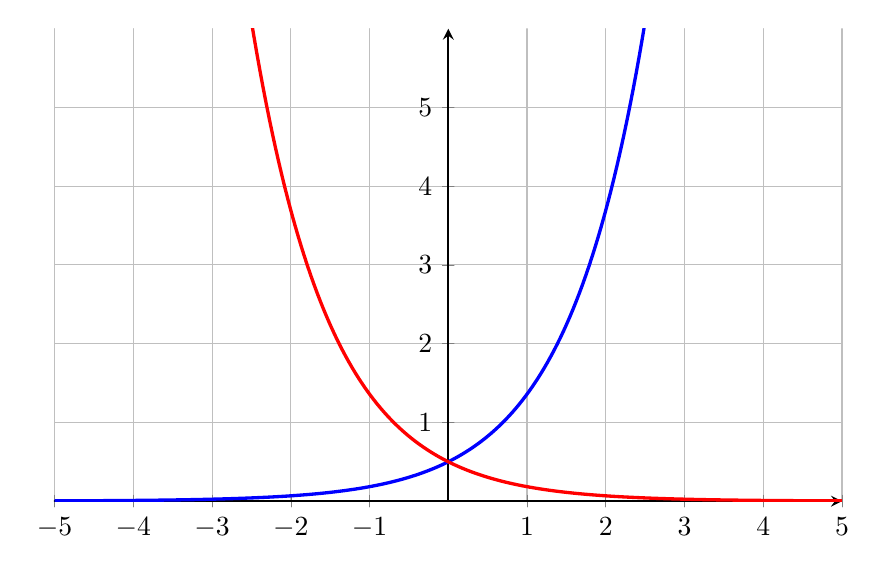
\begin{tikzpicture}[samples=250, line cap=round,line join=round,>=triangle 45,x=1cm,y=1cm]
		\begin{axis}[
			x=1cm,y=1cm,
			axis lines=middle,
			ymajorgrids=true,
			xmajorgrids=true,
			xmin=-5,
			xmax=5,
			ymin=-0,
			ymax=6,
			xtick={-7,-6,...,10},
			ytick={-4,-3,...,5},]
			\addplot[very thick, blue] plot(\x, {0.5*exp(\x)});
			\addplot[very thick, red] plot(\x, {0.5*exp(-\x)});
		\end{axis}
	\end{tikzpicture}
	\caption*{Graphs of \color{blue}$\frac{e^x}{2}$ and \color{red}$\frac{e^{-x}}{2}$}
\end{figure}
Now, we see,
	\begin{figure}[h]
	\centering
	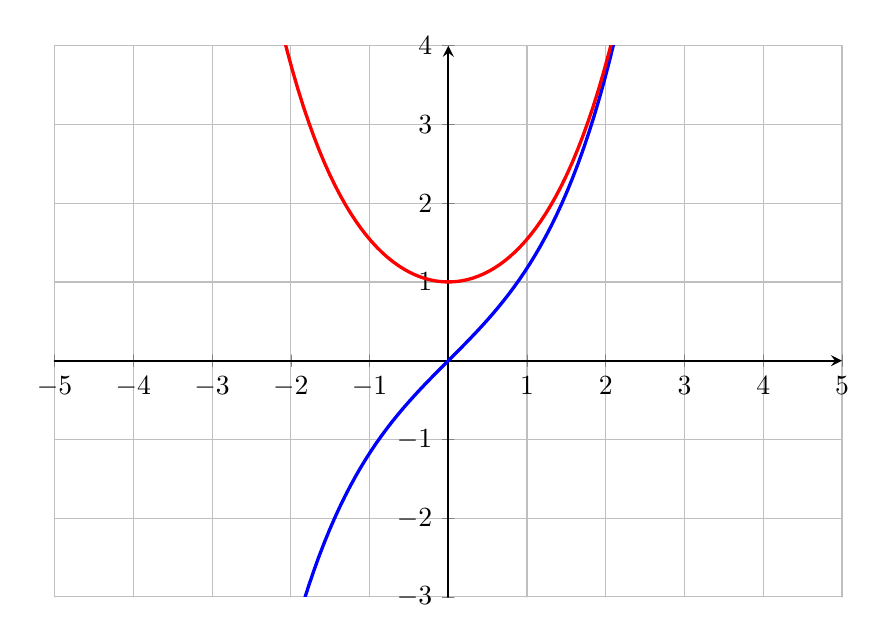
\begin{tikzpicture}[samples=150, line cap=round,line join=round,>=triangle 45,x=1cm,y=1cm]
		\begin{axis}[
			x=1cm,y=1cm,
			axis lines=middle,
			ymajorgrids=true,
			xmajorgrids=true,
			xmin=-5,
			xmax=5,
			ymin=-3,
			ymax=4,
			xtick={-10,-9,...,10},
			ytick={-10,-9,...,10},]
			\addplot[very thick, blue] plot(\x,{sinh(\x)});
			\addplot[very thick, red] plot(\x,{cosh(\x)});
		\end{axis}
	\end{tikzpicture}
	\caption*{Graphs of \color{blue}$\sinh x$ and \color{red}$\cosh x$}
\end{figure}
	\begin{figure}[h]
	\centering
	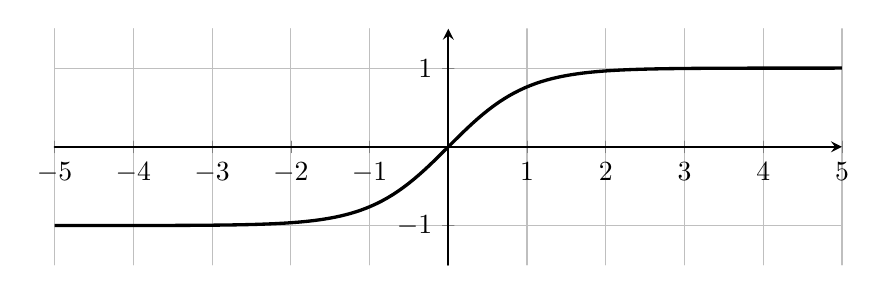
\begin{tikzpicture}[samples=150, line cap=round,line join=round,>=triangle 45,x=1cm,y=1cm]
		\begin{axis}[
			x=1cm,y=1cm,
			axis lines=middle,
			ymajorgrids=true,
			xmajorgrids=true,
			xmin=-5,
			xmax=5,
			ymin=-1.5,
			ymax=1.5,
			xtick={-10,-9,...,10},
			ytick={-10,-9,...,10},]
			\addplot[very thick, black] plot(\x,{tanh(\x)});
		\end{axis}
	\end{tikzpicture}
	\caption*{Graph of $\tanh x$}
\end{figure}
	\begin{figure}[H]
	\centering
	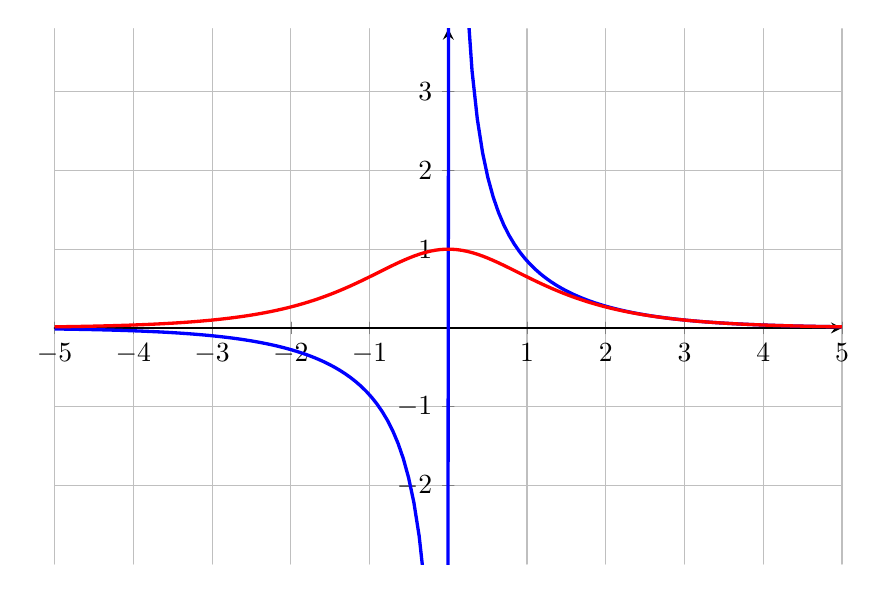
\begin{tikzpicture}[samples=150, line cap=round,line join=round,>=triangle 45,x=1cm,y=1cm]
		\begin{axis}[
			x=1cm,y=1cm,
			axis lines=middle,
			ymajorgrids=true,
			xmajorgrids=true,
			xmin=-5,
			xmax=5,
			ymin=-3,
			ymax=3.8,
			xtick={-10,-9,...,10},
			ytick={-2,...,10},]
			\addplot[very thick, blue] plot(\x,{1/sinh(\x)});
			\addplot[very thick, red] plot(\x,{1/cosh(\x)});
		\end{axis}
	\end{tikzpicture}
	\caption*{Graphs of \color{blue}$\csch x$ and \color{red}$\sech x$}
\end{figure}
\begin{figure}[H]
	\centering
	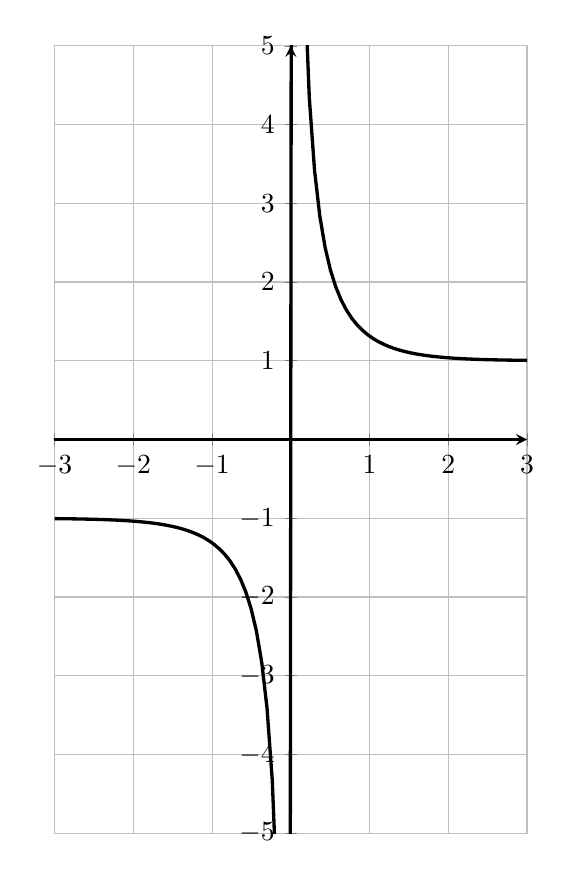
\begin{tikzpicture}[samples=150, line cap=round,line join=round,>=triangle 45,x=1cm,y=1cm]
		\begin{axis}[
			x=1cm,y=1cm,
			axis lines=middle,
			ymajorgrids=true,
			xmajorgrids=true,
			xmin=-3,
			xmax=3,
			ymin=-5,
			ymax=5,
			xtick={-10,-9,...,10},
			ytick={-10,-9,...,10},]
			\addplot[very thick, black] plot(\x,{1/tanh(\x)});
		\end{axis}
	\end{tikzpicture}
	\caption*{Graph of $\coth x$}
\end{figure}
\subsection{Identities of Conversion}
\[\begin{split}
	\sin(ix)&=i\sinh x\\
	\cos(ix)&=\cosh x\\
	\tan(ix)&=i\tanh x
\end{split}\]
For any identity $f(\sin x,\cos x)$, $f(i\sinh x, \cosh x)$ is also valid.
\subsection{Period}
Hyperbolic functions have no period in $\mathbb{R}$, however in $\mathbb{C}$,\begin{itemize}
	\item $\sinh x$ and $\cosh x$ have period $2in\pi$
	\item $\tanh x$ has period $in\pi$
\end{itemize}
\subsection{Inverse Hyperbolic Functions}
\[\sinh(x+iy)=u+iv\implies x+iy=\sinh^{-1}(u+iv)\]
Also, for the general solution,
\[\text{Sinh}^{-1}(u+iv)=2n\pi i+x+iy\]
\begin{eg}
	Show that $\sinh^{-1}z=\ln(z+\sqrt{z^2+1})$.
\end{eg}
\begin{explanation}
	Let $\sinh^{-1}z=w$,
	\[\implies z=\sinh w\, \land \, \cosh w=\sqrt{z^2+1}\]
	Also,
	\[\begin{split}
		\sinh w+\cosh w&=e^w\\
		\implies w&=\ln(z+\sqrt{z^2+1})\\
		\therefore \sinh^{-1}z&=\ln(z+\sqrt{z^2+1})
	\end{split}\]
	Similarly,
	\[\begin{split}
		\cosh^{-1}z&=\ln(z+\sqrt{z^2-1})\\
		\tanh^{-1}z&=\frac{1}{2}\ln(\frac{1+z}{1-z})
	\end{split}\]
\end{explanation}
\subsection{More Identities of Conversion}
\[\begin{split}
	\sinh^{-1}x&=-i\sin^{-1}ix\\
	\cosh^{-1}x&=-i\cos^{-1}x\\
	\tanh^{-1}x&=-i\tan^{-1}ix
\end{split}\]
\chapter{Functions of Several Variables}
First, we say that the real line $\mathbb{R}$ is both open and closed.
\begin{eg}
	$f:\mathbb{R}^2\to\mathbb{R}$ is given as,
	\[f(x,y)=xy\]
	Then the domain and range of $f$ is?
\end{eg}
\begin{explanation}
	Clearly,
	\[\text{Dom}(f)=\mathbb{R}^2\,\land \, \text{Ran}(f)=\mathbb{R}\]
\end{explanation}
\begin{eg}
	$f:\mathbb{R}^2\to\mathbb{R}$ is given as,
	\[f(x,y)=\frac{1}{x^2+y^2}\]
	Then the domain and range of $f$ is?
\end{eg}
\begin{explanation}
	Clearly,
	\[x^2+y^2>0\implies \frac{1}{x^2+y^2}<\infty\]
	Thus,
	\[\text{Dom}(f)=\mathbb{R}^2-{(0,0)}\,\land \, \text{Ran}(f)=\mathbb{R}^+\]
\end{explanation}
\begin{eg}
	$f:\mathbb{R}^2\to\mathbb{R}$ is given as,
	\[f(x,y)=\frac{1}{\sqrt{4-x^2-y^2}}\]
	Then the domain and range of $f$ is?
\end{eg}
\begin{explanation}
	Clearly,
	\[4-x^2-y^2>0\implies x^2+y^2<4\]
	Thus,
	\[\text{Dom}(f)=\{(x,y)| x^2+y^2<4\} \, \land \, \text{Ran}(f)=[\frac{1}{2},\infty)\]
\end{explanation}
\section{Limit in Higher Dimensions}
The limit of a function exists if on approaching the point from all directions from all possible paths, the same value is obtained.\\
Let there be $f:S\subseteq \mathbb{R}^2\to \mathbb{R}$, where, $f$ may or may not be defined at $(a,b)$, then,
\[\lim\limits_{(x,y)\to(a,b)} f(x,y)=L\]
\[\forall \epsilon>0 \exists \delta>0 (\begin{array}{l}
	\sqrt{(x-a)^2+(y-b)^2}<\delta\\
	|x-a|<\delta, |y-b|<\delta\\
	|x-a|+|y-b|<\delta
\end{array})\implies |f(x,y)-L|<\epsilon\]
\begin{eg}
	Find the limit of
	\[f(x,y)=\frac{xy}{x^2+y^2}\]
\end{eg}
\begin{explanation}
	Let $y=mx$ be the path on which $(0,0)$ lies.
	\[f(x,mx)=\frac{m}{1+m^2}\]
	Since the value of the function depends upon the path,
	\[\lim\limits_{(x,y)\to(0,0)}\frac{xy}{x^2+y^2} \text{Does not exist}\]
\end{explanation}
\section{Continuity}
Consider a function $f$ such that,
\[\lim\limits_{(x,y)\to(a,b)}f(x,y)=L\]
Then $f$ is continuous at a point $(a,b)$, is $f(x,y)$ is defined at $(a,b)$ and $L=f(a,b)$.
\begin{eg}
	Discuss the continuity of
	\[f(x,y)=\begin{cases}
		x^2+2y &, (x,y)\neq(1,2)\\
		0 &, (x,y)=(1,2) 
	\end{cases}\]
\end{eg}
\begin{explanation}
	Here,
	\[\lim\limits_{(x,y)\to(1,2)}f(x,y)=5\]
	Thus, the function is discontinuous.\\
	However, it is a removal point of discontinuity since it can be made continuous by changing the function definition.
\end{explanation}
\begin{eg}
	Show that $f$ is continuous at $(0,0)$,
	\[f(x)=\begin{cases}
		\frac{xy}{\sqrt{x^2+y^2}} &, (x,y)\neq(0,0)\\
		0 &, (x,y)=(0,0)
	\end{cases}\]
\end{eg}
\begin{explanation}
	Suppose $\epsilon>0$. Now choose $\delta=2\epsilon$.\\
	Let, $\sqrt{|x|^2+|y|^2}<\delta$.
	Check,
	\[\begin{split}
		|f(x,y)-f(0,0)|&=|\frac{xy}{\sqrt{x^2+y^2}}|\\
		&\leq \frac{1}{2}\sqrt{x^2+y^2} \quad (\because |xy|\leq \frac{x^2+y^2}{2})\\
		&\leq \frac{\delta}{2}=\epsilon
	\end{split}\]
\end{explanation}
Now, if the repeated limit exists, then the limit may or may not exist, however if the limit exists, then the repeated limit must exist, i.e.,
\[\lim\limits_{(x,y)\to(a,b)}f(x,y)=L\implies \lim\limits_{x\to a}\left(\lim\limits_{y\to b}f(x,y)\right)=\lim\limits_{y\to b}\left(\lim\limits_{x\to a}f(x,y)\right)=L\]
\section{Partial Derivatives}
The partial derivative of a function $f$ w.r.t $x$ at the point $(a,b)$ is,
\[f_x(a,b)=\eval{\pdv{f}{x}}_{(a,b)}=\pdv{f(a,b)}{x}=\lim\limits_{h\to0}\frac{f(a+h,b)-f(a,b)}{h}\]
It is possible that a function is discontinuous at some point but its partial derivative exists.\footnote{For the mixed partial derivatives to be equal, the first partial derivatives must exist and be continuous.}\\
\begin{eg}
	Find the partial derivative at $(0,0)$,
	\[f(x,y)=\begin{cases}
		\frac{xy}{x^2+y^2} &, (x,y)\neq(0,0)\\
		0 &, (x,y)=(0,0)
	\end{cases}\]
\end{eg}
\begin{explanation}
	\[\pdv{f(0,0)}{x}=\lim\limits_{h\to0}\frac{f(h,0)-0}{h}=0\]
	Hence, clearly the function is discontinuous at $(0,0)$ but the partial derivative exists.
\end{explanation}

\begin{eg}
	Given,
	\[f(x,y)=7x^2y^3+9xy^2+8xy+20e^x\cos y\]
	Find $\pdv{f}{x}$, $\pdv{f}{y}$, $\pdv[2]{f}{x}$, $\pdv[2]{f}{y}$, $\pdv{f}{x}{y}$, $\pdv{f}{y}{x}$.
\end{eg}
\begin{explanation}
	\[\begin{split}
		f_x(x,y)&=\pdv{f}{x}=14xy^3+9y^2+8y+20e^x\cos y\\
		f_y(x,y)&=\pdv{f}{y}=21x^2y^2+18xy+8x-20e^x\sin y\\
		f_{xx}(x,y)&=\pdv[2]{f}{x}=14y^3+20e^x\cos y\\
		f_{yy}(x,y)&=\pdv[2]{f}{y}=42x^2y+18x-20e^x\cos y\\
		f_{xy}(x,y)&=\pdv{f}{x}{y}=\pdv{x}\left(\pdv{f}{y}\right)=42xy^2+18y+8-20e^x\sin y\\
		f_{yx}(x,y)&=\pdv{f}{y}{x}=\pdv{y}\left(\pdv{f}{x}\right)=42xy^2+18y+8-20e^x\sin y\\
	\end{split}\]
\end{explanation}
\begin{eg}
	\[f(x,y,z)=\sqrt{x^2+y^2+z^2}\]
	Show that, $\pdv[2]{f}{x}+\pdv[2]{f}{y}+\pdv[2]{f}{z}=0$
\end{eg}
\begin{explanation}
	\[\pdv{f}{x}=\frac{x}{\sqrt{x^2+y^2+z^2}}\implies \pdv[2]{f}{x}=\frac{y^2+z^2}{(x^2+y^2+z^2)^\frac{3}{2}}\]
	Similarly,
	\[\pdv[2]{f}{y}=\frac{z^2+x^2}{(x^2+y^2+z^2)^\frac{3}{2}} \land \pdv[2]{f}{z}=\frac{x^2+y^2}{(x^2+y^2+z^2)^\frac{3}{2}}\]
\end{explanation}
\section{Composition of Functions}
Consider a function $z=f(x,y)$ and $x=g(t)$ and $y=h(t)$, then,
\[\dv{z}{t}=\pdv{z}{x}\dv{x}{t}+\pdv{z}{y}\dv{y}{t}\]
\begin{eg}
	\[z=e^{xy^2}\land x=t\cos t\land t\sin t\]
	Calculate $\dv{z}{t}\vert_{t=\frac{\pi}{2}}$.
\end{eg}
\begin{explanation}
	Clearly,
	\[\begin{split}
		\dv{z}{t}&=\pdv{z}{x}\dv{x}{t}+\pdv{z}{y}\dv{y}{t}\\
		&=y^2e^{xy^2}[\cos t-t\sin t]+2xye^{xy^2}[\sin t+t\cos t]\\
		\therefore \dv{z}{t}\vert_{t=\frac{\pi}{2}}&=-\frac{\pi^3}{8}
	\end{split}\]
\end{explanation}
\begin{theorem}[Euler's Theorem for Homogeneous Functions]
	If $f(x,y)$ is a homogeneous function of degree $n$, then,
	\[\begin{split}
		x\pdv{f}{x}+y\pdv{f}{y}&=nf\\
		x^2\pdv[2]{f}{x}+2xy\pdv{f}{x}{y}+y^2\pdv[2]{f}{y}&=n(n-1)f
	\end{split}\]
\end{theorem}
\begin{eg}
	Given,
	\[\ln u=\frac{x^3+y^3}{3x+4y}\]
	Then find the value of $x\pdv{f}{x}+y\pdv{f}{y}$.
\end{eg}
\begin{explanation}
	Let $z=\ln u$. Using Euler's Theorem,
	\[x\pdv{z}{x}+y\pdv{z}{y}=2z\]
	Now,
	\[\pdv{z}{x}=\pdv{z}{u}\pdv{u}{x} \land \pdv{z}{y}=\pdv{z}{u}\pdv{u}{y}\]
\end{explanation}
\begin{eg}
	Given,
	\[u=\sin^{-1}\left(\frac{x+2y+3z}{x^8+y^8+z^8}\right)\]
	Then prove that,
	\[x\pdv{u}{x}+y\pdv{u}{y}+z\pdv{u}{z}=-7\tan u\]
\end{eg}
\begin{explanation}
	Let $f=\sin u$. Using Euler's Theorem,
	\[\begin{split}
		x\pdv{f}{x}+y\pdv{f}{y}+z\pdv{f}{z}&=-7f\\
		\implies x\pdv{f}{u}\pdv{u}{x}+y\pdv{f}{u}\pdv{u}{y}+z\pdv{f}{u}\pdv{u}{z}&=-7\sin u\\
		\therefore x\pdv{u}{x}+y\pdv{u}{y}+z\pdv{u}{z}&=-7\tan u \quad \left(\pdv{f}{u}=\cos u\right)
	\end{split}\]
\end{explanation}
\section{Jacobian}
Consider two functions $u(x,y)$ and $v(x,y)$, then the Jacobian\footnote{Jo niche hai voh operator mein jaega, matlab w.r.t. whom} of $u,v$ w.r.t. $x,y$ is,
\[\mathbb{J}(x,y)=\frac{\partial{(u,v)}}{\partial{(x,y)}}=\begin{vmatrix}
	\pdv{u}{x} & \pdv{u}{y}\\
	\pdv{v}{x} & \pdv{v}{y}
\end{vmatrix}\]
Moreover, composition of Jacobian works as, if $u(r,s)$ and $v(r,s)$ where $r=f(x,y)$ and $s=g(x,y)$,
\[\frac{\partial(u,v)}{\partial(x,y)}=\frac{\partial(u,v)}{\partial(r,s)}\frac{\partial(r,s)}{\partial(x,y)}\]
\begin{eg}[Polar Coordinates]
	If $x=r\cos\theta$ and $y=r\sin\theta$, then find $\mathbb{J}(r,\theta)$.
\end{eg}
\begin{explanation}
	\[\mathbb{J}(r,\theta)=\begin{vmatrix}
		\cos\theta & -r\sin\theta\\
		\sin\theta & r\cos\theta
	\end{vmatrix}=r\]
\end{explanation}
\begin{eg}[Cylindrical Coordinates]
	If $x=r\cos\theta$, $y=r\sin\theta$ and $z=z$, then find $\mathbb{J}(r,\theta,z)$.
\end{eg}
\begin{explanation}
	\[\mathbb{J}(r,\theta, z)=r\]
\end{explanation}
\begin{eg}[Spherical Coordinates]
	If $x=r\sin\theta\cos\phi$, $y=r\sin\theta\sin\phi$ and $z=r\cos\theta$ where $\theta\in [0,2\pi]\land \phi\in[0,\pi]$, then find $\mathbb{J}(r,\theta,\phi)$.
\end{eg}
\begin{explanation}
	\[\mathbb{J}(r,\theta,\phi)=r^2\sin\theta\]
\end{explanation}
\section{Explicit and Implicit Functions}
A function $f$ is said to be explicit if one variable can be represented in terms of other variables.\\
If $f$ is implicit, such that $f(x,y)=c$, then $\dv{y}{x}=-\frac{f_x}{f_y}$.
\begin{theorem}[Taylor's Theorem]
	\[f(x,y)=f(a,b)+(x-a)\pdv{f(a,b)}{x}+(y-b)\pdv{f(a,b)}{y}+\frac{1}{2!}\left[(x-a)\pdv{x}+(y-b)\pdv{y}\right]^2f(a,b)+\ldots +R_n\]
	Where,
	\[R_n=\frac{1}{(n+1)!}\left[(x-a)\pdv{x}+(y-b)\pdv{y}\right]^{n+1}f(a+\theta(x-a),b+\phi(y-b)) \quad (\theta,\phi\in (0,1))\]
\end{theorem}
\begin{eg}
	\[f(x,y)=x^3+x^2y+xy^2+y^2\]
	Express $f$ in powers of $(x-1)$ and $(y+2)$.
\end{eg}
\begin{explanation}
	Here, $a=1,b=-2$,
	Thus,
	\[f(1,-2)=7\implies f_x(1,-2)=3\land f_y(1,-2)=-7\implies f_{xx}(1,-2)=2\land f_{yy}(1,-2)=4\land f_{xy}(1,-2)=-2\]
	Also,
	\[f_{xxy}=6\land f_{yyy}=0\land f_{xxy}=2\land f_{yyx}=2\]
	\[\begin{split}
		f(x,y)&=7+3(x-1)+(-7)(y+2)+\frac{1}{2!}\left[2(x-1)^2+4(y+2)^2+(-2)(x-1)(y+2)\right]+\\
		&\frac{1}{3!}\left[6(x-1)^3+3(2)(x-1)^2(y+2)+3(2)(x-1)(y+2)^2\right]\\
		\therefore f(x,y)&=7+3(x-1)-7(y+2)+(x-1)^2+2(y+2)^2-(x-1)(y+2)+(x-1)^3+(x-1)^2(y+2)+(x-1)(y+2)^2
	\end{split}\]
\end{explanation}
\section{Maxima and Minima of Two Variables}
A function $f(x,y)$ is said to obtain minimum value of $f$ at point $(a,b)$, if there exists a neighborhood ($N$) of $(a,b)$ such that $f(a,b)<f(x,y)$ for all $(x,y)\in N$.\\
A function $f(x,y)$ is said to obtain maximum value of $f$ at point $(a,b)$, if there exists a neighborhood ($N$) of $(a,b)$ such that $f(a,b)>f(x,y)$ for all $(x,y)\in N$.
\subsection{Critical Point}
Any point $(a,b)$ is said to be a critical point of $f$ if $\begin{cases}
	\pdv{f(a,b)}{x}=0\\
	\pdv{f(a,b)}{y}=0
\end{cases}$
\[A=\pdv[2]{f}{x}\land B=\pdv{f}{x}{y}\land C=\pdv[2]{f}{y}\]
\[\begin{cases}
	AC-B^2>0 &, \begin{cases}
		A>0 &, \text{minima}\\
		A<0 &, \text{maxima}
	\end{cases} \\
	AC-B^2<0 &, \text{neither max nor min, i.e. saddle point}\\
	AC-B^2=0 &, \text{Further investigation}
\end{cases}\]
\begin{eg}
	\[f(x,y)=(x-y)^2\]
\end{eg}
\begin{explanation}
	\[\pdv{f}{x}=0\land \pdv{f}{y}=0\implies x=y\]
	Critical points are $S=\{x\in\mathbb{R}|(x,x)\}$.
	\[f_{xx}=2\land f_{xy}=-2\land f_{yy}=2\implies AC-B^2=0\]
	Clearly, at $S$ is set of minima.
\end{explanation}
\begin{eg}
	\[f(x,y)=x^4+y^4-2x^2-2y^2+4xy\]
\end{eg}
\begin{explanation}
	\[\begin{split}
		f_x&=4x^3-4x+4y=0\\
		f_y&=4y^3-4y+4x=0
	\end{split}\]
	Thus, $x=-y$ and $(x,y)=\{(0,0),(\sqrt{2},-\sqrt{2}),(-\sqrt{2},\sqrt{2})\}$.
	\[f_{xx}=12x^2-4\land f_{xy}=4\land f_{yy}=12y^2-4\]
	At $(0,0)$, $AC-B^2=0$\\
	At $(\sqrt{2},-\sqrt{2})$, $AC-B^2>0\land A>0$\\
	At $(-\sqrt{2},\sqrt{2})$, $AC-B^2>0\land A>0$\\
	Thus, $(\sqrt{2},-\sqrt{2})$ and $(-\sqrt{2},\sqrt{2})$ are points of minima.\\
	For $(0,0)$, along $x$,
	\[y=0\]
\end{explanation}



\section{Tutorial-3}
\subsection{Determine the domain and range of the following functions}
\begin{asign}
	\[f(x,y)=\frac{1}{x-y}\]
\end{asign}
\begin{anse}
	Here,
	\[x-y\neq0\implies x\neq y\]
	Thus, the domain is,
	\[\text{Dom}(f)=\mathbb{R}^2-\{x,y \in \mathbb{R}| x= y\}\]
\end{anse}
\begin{asign}
	\[f(x,y,z)=\sqrt{1-x^2-y^2-z^2}\]
\end{asign}
\begin{anse}
	Here,
	\[1-x^2-y^2-z^2\geq 0\implies x^2+y^2+z^2\leq1\]
	Thus,
	\[\text{Dom}(f)=\{x,y,z\in \mathbb{R} | x^2+y^2+z^2\leq1\}\]
\end{anse}
\begin{asign}
	\[f(x,y)=\sqrt{16-4x^2-y^2}\]
\end{asign}
\begin{anse}
	Here,
	\[16-4x^2-y^2\geq0\implies4x^2+y^2\leq16\]
	Thus,
	\[\text{Dom}(f)=\{x,y\in\mathbb{R}| 4x^2+y^2\leq16\}\]
\end{anse}
\begin{asign}
	\[f(x,y)=\frac{\sqrt{4-x^2}}{y^2+3}\]
\end{asign}
\begin{anse}
	Here,
	\[4-x^2\geq0\implies x^2\leq4\implies x\in[-2,2]\]
	Thus,
	\[\text{Dom}(f)=\{x,y\in\mathbb{R}| x\in[-2,2]\}\]
\end{anse}
\subsection{Examine if the limits of the following functions $f(x,y)$ as $(x,y)\to(0,0)$ exist}
\begin{asign}
	\[f(x,y)=\begin{cases}
		\frac{x^2+y^2}{x^2-y^2} &, x\neq y\\
		0 &, x=y
	\end{cases}\]
\end{asign}
\begin{anse}
	Let the path of choice be $y=mx$,
	\[\lim\limits_{(x,y)\to(0,0)}f(x,y)=\frac{1-m^2}{1+m^2}\]
	Since the limit depends on the path, $f(x,y)$ is not continuous at $(0,0)$.
\end{anse}
\begin{asign}
	\[f(x,y)=xy\left(\frac{x^2-y^2}{x^2+y^2}\right)\]
\end{asign}
\begin{anse}
	Suppose $\epsilon>0$. Now choose $\delta=\sqrt{2\epsilon}$.
	Let $\sqrt{x^2+y^2}<\delta$. Check,
	\[\begin{split}
		|f(x,y)|&=|xy\frac{x^2-y^2}{x^2+y^2}|\\
		&<|xy| \quad \left(\because \frac{x^2-y^2}{x^2+y^2}<1\right)\\
		&<\frac{1}{2}(x^2+y^2)\\
		&<\frac{\delta^2}{2}=\epsilon
	\end{split}\]
\end{anse}
\begin{asign}
	\[f(x,y)=\begin{cases}
		x\sin\frac{1}{y}+y\sin\frac{1}{x} &, xy\neq0\\
		0 &, xy=0
	\end{cases}\]
\end{asign}
\begin{anse}
		Suppose $\epsilon>0$. Now choose $\delta=\epsilon$.\\
	Let $|x|+|y|<\delta$. Check,
	\[\begin{split}
		|f(x,y)-f(0,0)|&=|x\sin\frac{1}{y}+y\sin\frac{1}{x} -0|\\
		&\leq | x\sin\frac{1}{y}|+|y\sin\frac{1}{x} |\\
		&\leq |x|+|y|\\
		&< \delta=\epsilon
	\end{split}\]
\end{anse}
\begin{asign}
	\[f(x,y)=\frac{\sin(xy)}{x^2+y^2}\]
\end{asign}
\begin{anse}
	Let the path of choice be $y=mx$,
	\[\lim\limits_{(x,y)\to(0,0)}f(x,y)=\frac{m}{1+m^2}\]
	Since the limit depends on the path, $f(x,y)$ is not continuous at $(0,0)$.
\end{anse}
\subsection{Examine the continuity of the following functions at $(0,0)$}
\begin{asign}
	\[f(x,y)=\begin{cases}
		\frac{xy^3}{x^2+y^6} &, (x,y)\neq(0,0)\\
		0 &, \text{otherwise}
	\end{cases}\]
\end{asign}
\begin{anse}
	Let the path of choice be $y^3=mx$, thus,
	\[\lim\limits_{(x,y)\to(0,0)}f(x,y)=\frac{m}{1+m^2}\]
	Since the limit depends on the path, $f(x,y)$ is not continuous at $(0,0)$.
\end{anse}
\begin{asign}
	\[f(x,y)=\begin{cases}
		x^2+y^2 &, 	x^2+y^2\leq 1\\
		0 &, \text{otherwise}
	\end{cases}\]
\end{asign}
\begin{anse}
	Suppose $\epsilon>0$. Now choose, $\delta=\sqrt{\frac{\epsilon}{2}}$. Let $|x|<\delta\land |y|<\delta$. Check,
	\[\begin{split}
		|f(x,y)|&=|x^2+y^2|\\
		&\leq |x|^2+|y|^2\\
		&\leq 2\delta^2\\
		&=\epsilon
	\end{split}\]
\end{anse}
\begin{asign}
	\[f(x,y)=\begin{cases}
		\frac{\sin^2(x-y)}{|x|+|y|} &, (x,y)\neq(0,0)\\
		0 &, \text{otherwise}
	\end{cases}\]
\end{asign}
\begin{anse}
	Suppose $\epsilon>0$, Now choose $\delta=\epsilon$. Let $|x|+|y|<\delta$. Check,
	\[\begin{split}
		|f(x,y)|&=\left|\frac{\sin^2(x-y)}{|x|+|y|}\right|\\
		&\leq \left|\frac{|x-y|^2}{|x|+|y|}\right|\\
		&\leq |x|+|y| \quad (\because |x-y|^2 \leq (|x|+|y|)^2)\\
		&<\delta=\epsilon
	\end{split}\]
\end{anse}
\begin{asign}
	Find the partial derivative of the function $f(x,y,z)=\ln(x^2+2y+z^3)$.
\end{asign}
\begin{anse}
	W.r.t. $x$,
	\[\pdv{f}{x}=\frac{2x}{x^2+2y+z^3}\]
	W.r.t. $y$,
	\[\pdv{f}{y}=\frac{2}{x^2+2y+z^3}\]
	W.r.t. $z$,
	\[\pdv{f}{x}=\frac{3z^2}{x^2+2y+z^3}\]
\end{anse}
\begin{asign}
	Show that the function $u=\ln(\sqrt{x^2+y^2})$ satisfy the Laplace equation $\left(\pdv[2]{u}{x}+\pdv[2]{u}{y}=0\right)$.
\end{asign}
\begin{anse}
	Clearly,
	\[\pdv{u}{x}=\frac{x}{x^2+y^2}\implies \pdv[2]{u}{x}=\frac{y^2-x^2}{x^2+y^2}\]
	By symmetry,
	\[\pdv[2]{u}{y}=\frac{x^2-y^2}{x^2+y^2}\]
	Thus,
	\[\pdv[2]{u}{x}+\pdv[2]{u}{y}=0\]
\end{anse}
\subsection{Find the first order partial derivatives of the following functions at the given points}
\begin{asign}
	\[f(x,y)=(3x^3+2xy)^3\quad (2,0)\]
\end{asign}
\begin{anse}
	W.r.t. $x$,
	\[\pdv{f}{x}=3(3x^3+2xy)^2(9x^2+2y)\implies \eval{\pdv{f}{x}}_{(2,0)}=2592\]
	W.r.t $y$,
	\[\pdv{f}{y}=3(3x^3+2xy)^2(2x)\implies\eval{\pdv{f}{y}}_{(2,0)}=288\]
\end{anse}
\begin{asign}
	\[f(x,y)=\left(\frac{4x^2+2y^2}{xy}\right)\quad (\sqrt{3},\sqrt{2})\]
\end{asign}
\begin{anse}
	Simplifying,
	\[f(x,y)=2\cdot\left(\frac{2x}{y}+\frac{y}{x}\right)\]
	W.r.t. $x$,
	\[\pdv{f}{x}=2\left(\frac{2}{y}-\frac{y}{x^2}\right)\implies\eval{\pdv{f}{x}}_{(\sqrt{3},\sqrt{2})}=\frac{4\sqrt{2}}{3}\]
	W.r.t. $y$,
	\[\pdv{f}{y}=2\left(\frac{-2x}{y^2}+\frac{1}{x}\right)\implies \eval{\pdv{f}{y}}_{(\sqrt{3},\sqrt{2})}=-\frac{4\sqrt{3}}{3}\]
\end{anse}
\subsection{Calculate the partial derivatives of the following functions at $(0,0)$}
\begin{asign}
	\[f(x,y)=\begin{cases}
		x\sin\frac{1}{x}+y\sin\frac{1}{y} &, xy\neq0\\
		0 &, xy=0
	\end{cases}\]
\end{asign}
\begin{anse}
	W.r.t. $x$,
	\[\begin{split}
		\pdv{f}{x}&=\lim\limits_{h\to0}\frac{f(h,0)-f(0,0)}{h}\\
		&=0
	\end{split}\]
	Similarly for $y$.
\end{anse}
\begin{asign}
	\[f(x,y)=\begin{cases}
		\frac{xy}{x^2+y^2} &, x^2+y^2\neq0\\
		0 &, x=y=0
	\end{cases}\]
\end{asign}
\begin{anse}
	W.r.t. $x$,
	\[\begin{split}
		\pdv{f}{x}&=\lim\limits_{h\to0}\frac{f(h,0)-f(0,0)}{h}\\
		&=0 
	\end{split}\]
	Similarly for $y$.
\end{anse}
\begin{asign}
	\[f(x,y)=\begin{cases}
		\frac{x^6-2y^4}{x^2+y^2} &, x^2+y^2\neq0\\
		0 &, x=y=0
	\end{cases}\]
\end{asign}
\begin{anse}
	W.r.t. $x$,
	\[\begin{split}
		\pdv{f}{x}&=\lim\limits_{h\to0}\frac{f(h,0)-f(0,0)}{h}\\
		&=\lim\limits_{h\to0}\frac{h^6}{h^2}\\
		&=0
	\end{split}\]
	W.r.t. $y$,
	\[\begin{split}
		\pdv{f}{y}&=\lim\limits_{k\to0}\frac{f(0,k)-f(0,0)}{k}\\
		&=\lim\limits_{k\to0} \frac{-2k^4}{k^2}\\
		&=0
	\end{split}\]
\end{anse}
\begin{asign}
	\[f(x,y)=\begin{cases}
		y\sin\frac{1}{x} &, x\neq0\\
		0 &, x=0
	\end{cases}\]
\end{asign}
\begin{anse}
	W.r.t. $x$,
	\[\begin{split}
		\pdv{f}{x}&=\lim\limits_{h\to0}\frac{f(h,0)-f(0,0)}{h}\\
		&= \text{Not defined}
	\end{split}\]
	W.r.t. $y$,
	\[\begin{split}
		\pdv{f}{y}&=\lim\limits_{k\to0}\frac{f(0,k)-f(0,0)}{k}\\
		&=0
	\end{split}\]
\end{anse}
\begin{asign}
	\[f(x,y)=\begin{cases}
		\frac{x^3+y^3}{x-y} &, x\neq y\\
		0 &, x=y
	\end{cases}\]
\end{asign}
\begin{anse}
	\[\begin{split}
		\pdv{f}{x}&=\lim\limits_{h\to0}\frac{f(h,0)-f(0,0)}{h}\\
		&=0
	\end{split}\]
	Similarly for $y$.
\end{anse}
\begin{asign}
	\[f(x,y)=\sqrt{|xy|}\]
\end{asign}
\begin{anse}
	\[\begin{split}
		\pdv{f}{x}&=\lim\limits_{h\to0}\frac{f(h,0)-f(0,0)}{h}\\
		&=0
	\end{split}\]
	Similarly for $y$.
\end{anse}
\begin{asign}
	If $F(x,y)=x^4y^2\sin^{-1}\frac{y}{x}$, then show that $x\pdv{F}{x}+y\pdv{F}{y}=6F$.
\end{asign}
\begin{anse}
	Checking the condition for homogeneity,
	\[F(\lambda x,\lambda y)=\lambda^6 F(x,y)\]
	Thus, using Euler's Theorem for Homogeneous Functions,
	\[x\pdv{F}{x}+y\pdv{F}{y}=6F\]
\end{anse}
\begin{asign}
	If $F=\tan^{-1}\left(\frac{x^3+y^3}{x-y}\right)$, then prove that, \begin{enumerate}
		\item $x\pdv{F}{x}+y\pdv{F}{y}=\sin2F$
		\item $x^2\pdv[2]{F}{x}+2xy\pdv{f}{F}{y}+y^2\pdv[2]{F}{y}=2\cos3F\sin F$
	\end{enumerate}
\end{asign}
\begin{anse}
	Let $\tan F=z=\frac{x^3+y^3}{x-y}$, here, checking the condition for homogeneity for $z$,
	\[z=y^2\frac{\left(\frac{x}{y}\right)^3+1}{\left(\frac{x}{y}\right)-1}\]
	Using Euler's Theorem for Homogeneous Functions on $z$,
	\[x\pdv{z}{x}+y\pdv{z}{y}=2z\]
	Moreover,
	\[\pdv{F}{x}=\frac{1}{\sec^2F}\pdv{z}{x} \land \pdv{F}{y}=\frac{1}{\sec^2F}\pdv{z}{y} \]
	Replacing,
	\[x\pdv{F}{x}+y\pdv{F}{y}=2\tan F \sec^2F=\sin 2F\]
	Differentiating w.r.t. $x$ and $y$, then multiplying with $x$ and $y$ respectively we get,
	\[\begin{split}
		x\pdv{F}{x}+x^2\pdv[2]{F}{x}+xy\pdv{F}{x}{y}&=2\cos2F\cdot x\pdv{F}{x}\\
		y\pdv{F}{y}+y^2\pdv[2]{F}{y}+xy\pdv{F}{x}{y}&=2\cos2F\cdot y\pdv{F}{y}\\
	\end{split}\]
	Adding the equations,
	\[x^2\pdv[2]{F}{x}+2xy\pdv{F}{x}{y}+y^2\pdv[2]{F}{y}=\sin4F-\sin2F=2\cos3F\sin F\]
\end{anse}
\begin{asign}
	If $F=\sin^{-1}\left(\frac{x+y}{\sqrt{x}+\sqrt{y}}\right)$, then prove that, \begin{enumerate}
		\item $x\pdv{F}{x}+y\pdv{F}{y}=\frac{1}{2}\tan F$
		\item $x^2\pdv[2]{F}{x}+2xy\pdv{F}{x}{y}+y^2\pdv[2]{F}{y}=-\frac{\sin F\cos 2F}{4\cos^3F}$
	\end{enumerate}
\end{asign}
\begin{anse}
	Let $\sin F=z=\frac{x+y}{\sqrt{x}+\sqrt{y}}$, here, checking the condition for homogeneity for $z$,
	\[z=y^\frac{1}{2}\left( \frac{x+y}{\sqrt{x}+\sqrt{y}} \right)\]
	Using Euler's Theorem for Homogeneous Functions on $z$,
	\[x\pdv{z}{x}+y\pdv{z}{y}=\frac{z}{2}\]
	Moreover,
	\[\pdv{F}{x}=\frac{1}{\cos F}\pdv{z}{x} \land \pdv{F}{y}=\frac{1}{\cos F}\pdv{z}{y} \]
	Replacing,
	\[x\pdv{F}{x}+y\pdv{F}{y}=\frac{1}{2}\tan F\]
	Differentiating w.r.t. $x$ and $y$, then multiplying with $x$ and $y$ respectively we get,
	\[\begin{split}
		x\pdv{F}{x}+x^2\pdv[2]{F}{x}+xy\pdv{F}{x}{y}&=\frac{1}{2}\sec^2 F\cdot x\pdv{F}{x}\\
		y\pdv{F}{y}+y^2\pdv[2]{F}{y}+xy\pdv{F}{x}{y}&=\frac{1}{2}\sec^2 F\cdot y\pdv{F}{y}\\
	\end{split}\]
	Adding the equations,
	\[x^2\pdv[2]{F}{x}+2xy\pdv{F}{x}{y}+y^2\pdv[2]{F}{y}=-\frac{\sin F\cos 2F}{4\cos^3F}\]
\end{anse}
\begin{asign}
	If $u=\tan^{-1}\frac{y^2}{x}$, then prove that $x^2\pdv[2]{u}{x}+2xy\pdv{u}{x}{y}+y^2\pdv[2]{u}{y}=-\sin^2u\sin2u$.
\end{asign}
\begin{anse}
	Let $\tan u=z=\frac{y^2}{z}$, here, checking the condition for homogeneity for $z$, we get $n=1$,
	Using Euler's Theorem for Homogeneous Functions on $z$,
	\[x\pdv{z}{x}+y\pdv{z}{y}=z\]
	Moreover,
	\[\pdv{u}{x}=\frac{1}{\sec^2u}\pdv{z}{x} \land \pdv{u}{y}=\frac{1}{\sec^2u}\pdv{z}{y} \]
	Replacing,
	\[x\pdv{u}{x}+y\pdv{u}{y}=\frac{\sin2u}{2}\]
	Differentiating w.r.t. $x$ and $y$, then multiplying with $x$ and $y$ respectively we get,
	\[\begin{split}
		x\pdv{u}{x}+x^2\pdv[2]{u}{x}+xy\pdv{f}{x}{y}&=\cos2u\cdot x\pdv{u}{x}\\
		y\pdv{F}{y}+y^2\pdv[2]{f}{y}+xy\pdv{f}{x}{y}&=\cos2u \cdot y\pdv{u}{y}\\
	\end{split}\]
	Adding the equations,
	\[x^2\pdv[2]{u}{x}+2xy\pdv{u}{x}{y}+y^2\pdv[2]{u}{y}=-\sin^2u\sin2u\]
\end{anse}
\begin{asign}
	If $u=u\left(\frac{x-y}{xy},\frac{z-x}{zx}\right)$, then show that $x^2\pdv{u}{x}+y^2\pdv{u}{y}+z^2\pdv{u}{z}=0$.
\end{asign}
\begin{anse}
	Let $\frac{x-y}{xy}=a$ and $\frac{z-x}{zx}=b$, thus,
	\[\begin{split}
		\pdv{u}{x}&=\pdv{u}{a}\pdv{a}{x}+\pdv{u}{b}\pdv{b}{x}=\frac{1}{x^2}\left(\pdv{u}{a}-\pdv{u}{b}\right)\\
		\pdv{u}{y}&=\pdv{u}{a}\pdv{a}{y}+\pdv{u}{b}\pdv{b}{y}=-\frac{1}{y^2}\pdv{u}{a}\\
		\pdv{u}{z}&=\pdv{u}{a}\pdv{a}{z}+\pdv{u}{b}\pdv{b}{z}=\frac{1}{z^2}\pdv{u}{b}
	\end{split}\]
	Adding,
	\[x^2\pdv{u}{x}+y^2\pdv{u}{y}+z^2\pdv{u}{z}=0\]
\end{anse}
\begin{asign}
	If $z=f(x,y)$ and $x=e^u\cos v$, $y=e^u\sin v$, prove that $x\pdv{z}{v}+y\pdv{z}{u}=e^{2u}\pdv{z}{y}$ and $\left(\pdv{z}{v}\right)^2+\left(\pdv{z}{u}\right)^2= e^{-2u}\left[ \left(\pdv{z}{x}\right)^2 + \left(\pdv{z}{y}\right)^2\right]$.
\end{asign}
\begin{anse}
	Clearly,
	\[\begin{split}
		\pdv{z}{v}&=\pdv{z}{x}\pdv{x}{v}+\pdv{z}{y}\pdv{y}{v}=\pdv{z}{x}(-e^u\sin v)+\pdv{z}{y}(e^u\cos v)  \\
		\pdv{z}{u}&=\pdv{z}{x}\pdv{x}{u}+\pdv{z}{y}\pdv{y}{u}=\pdv{z}{x}(e^u\cos v)+\pdv{z}{y}(e^u\sin v)
	\end{split}\]
	Multiplying and adding,
	\[x\pdv{z}{v}+y\pdv{z}{u}=e^{2u}\pdv{z}{y}\]
	Squaring and adding,
	\[\left(\pdv{z}{v}\right)^2+\left(\pdv{z}{u}\right)^2= e^{-2u}\left[ \left(\pdv{z}{x}\right)^2 + \left(\pdv{z}{y}\right)^2\right] \]
\end{anse}
\begin{asign}
	Show that $f_{xy}(0,0)\neq f_{yx}(0,0)$ for the function $f(x,y)$ defined by
	\[f(x,y)=\begin{cases}
		x^2\tan^{-1}\left(\frac{y}{x}\right)-y^2\tan^{-1}\left(\frac{x}{y}\right) &, (x,y)\neq (0,0)\\
		0 &, (x,y)= (0,0)
	\end{cases}\]
\end{asign}
\begin{anse}
	
\end{anse}
\subsection{Find the Jacobian of the following functions}
\begin{asign}
	\[u(x,y,z)=\frac{yz}{x} \; \land \; v(x,y,z)=\frac{zx}{y} \; \land \; w(x,y,z)=\frac{xy}{z}\]
\end{asign}
\begin{anse}
	The Jacobian is given by,
	\[\frac{\partial(u,v,w)}{\partial(x,y,z)}=\begin{vmatrix}
		\frac{-yz}{x^2} & \frac{z}{x} & \frac{y}{x}\\
		\frac{z}{y} & \frac{-zx}{y^2} & \frac{x}{y}\\
		\frac{y}{z} & \frac{x}{z} & \frac{-xy}{z^2}
	\end{vmatrix}=4\]
\end{anse}
\begin{asign}
	\[u(r,\theta)=r\cos2\theta \; \land \; v(r,\theta)=r\sin2\theta\]
\end{asign}
\begin{anse}
	The Jacobian is given by,
	\[\frac{\partial{(u,v)}}{\partial{(x,y)}}=\begin{vmatrix}
		\cos2\theta & -2r\sin\theta \\
		\sin2\theta & 2r\cos\theta
	\end{vmatrix}=2r\cos\theta \]
\end{anse}
\begin{asign}
	If $u=xyz$, $v=x^2+y^2+z^2$, $w=x+y+z$, find $\frac{\partial(x,y,z)}{\partial(u,v,w)}$.
\end{asign}
\begin{anse}
	First,
	\[\frac{\partial(u,v,w)}{\partial(x,y,z)}=\begin{vmatrix}
		yz & xz& xy\\
		2x& 2y & 2z\\
		1 & 1 & 1
	\end{vmatrix}=-2(x-y)(y-z)(z-x)\]
	Thus,
	\[\frac{\partial(x,y,z)}{\partial(u,v,w)}=\frac{1}{\frac{\partial(u,v,w)}{\partial(x,y,z)}}=\frac{-1}{2(x-y)(y-z)(z-x)}\]
\end{anse}
\begin{asign}
	If $x=u(1-v)$, $y=uv$, prove that $\mathbb{J}\mathbb{J}'=1$.
\end{asign}
\begin{anse}
	First calculating $\mathbb{J}=\frac{\partial(x,y)}{\partial(u,v)}=\begin{vmatrix}
	1-v & -u\\
	v & u
	\end{vmatrix}=u$.
	Moreover, 
	\[u=x+y \land v=\frac{y}{x+y}\]
	Thus,
	\[\mathbb{J}'=\frac{\partial(u,v)}{\partial(x,y)}=\begin{vmatrix}
		1 & 1\\
		\frac{-y}{(x+y)^2} & \frac{x}{(x+y)^2}
	\end{vmatrix}=\frac{1}{x+y}=\frac{1}{u}\]
	Hence, we can say that for the given set of variables,
	\[\mathbb{J}\mathbb{J}'=1\]
\end{anse}
\begin{asign}
	If $u=x^2-2y^2$,$v=2x^2-y^2$, where $x=r\cos\theta$, $y=r\sin\theta$, show that $\frac{\partial(u,v)}{\partial(r,\theta)}=6r^2\sin2\theta$.
\end{asign}
\begin{anse}
	\[\begin{split}
		\frac{\partial(u,v)}{\partial(r,\theta)}&=\frac{\partial(u,v)}{\partial(x,y)}\frac{\partial(x,y)}{\partial(r,\theta)}\\
		&=\begin{vmatrix}
			2x& -4y\\
			4x & -2y
		\end{vmatrix}r\\
		&=r(12xy)\\
		&=6r^3\sin2\theta
	\end{split}\]
\end{anse}
\begin{asign}
	If $u=x\sqrt{1-y^2}+y\sqrt{1-x^2}$, $v=\sin^{-1}x+\sin^{-1}y$, then show that $u$ and $v$ are functionally related and find the relationship.
\end{asign}
\begin{anse}
	Clearly,
	\[\sin^{-1}u=v\]
\end{anse}
\subsection{Find $f_u$, $f_v$ and total derivative for the functions}
\begin{asign}
	\[f(x,y)=e^x\cos y \; , x=ue^v \; y=u+v-1\]
\end{asign}
\begin{anse}
	Clearly,
	\[\begin{split}
		f_u&=\pdv{f}{x}\pdv{x}{u}+\pdv{f}{y}\pdv{y}{u}=e^x(e^v\cos y-\sin y)\\
		f_v&=\pdv{f}{x}\pdv{x}{v}+\pdv{f}{y}\pdv{y}{v}=e^x(ue^v\cos y-\sin y)
	\end{split}\]
	The total derivative is,
	\[\dd{f}=\pdv{f}{x}\dd{x}+\pdv{f}{y}\dd{y}=e^x\cos y\dd{x} -e^x\sin y\dd{y}\]
\end{anse}
\begin{asign}
	\[f(x,y)=xy \; , x=e^{2u}\cos v \; , v=e^u\sin v\]
\end{asign}
\begin{anse}
	Clearly,
	\[\begin{split}
		f_u&=\pdv{f}{x}\pdv{x}{u}+\pdv{f}{y}\pdv{y}{u}= 3xy \\
		f_v&=\pdv{f}{x}\pdv{x}{v}+\pdv{f}{y}\pdv{y}{v}= xy(\cos2v)
	\end{split}\]
	The total derivative is,
	\[\dd{f}=\pdv{f}{x}\dd{x}+\pdv{f}{y}\dd{y}=y\dd{x}+x\dd{y}\]
\end{anse}
\begin{asign}
	\[f(x,y)=x\sinh y + y\cosh x \; , x=u^2+1 \; ,y=v^2\]
\end{asign}
\begin{anse}
	Clearly,
	\[\begin{split}
		f_u&=\pdv{f}{x}\pdv{x}{u}+\pdv{f}{y}\pdv{y}{u}= 2u(\sinh y+y\sinh x) \\
		f_v&=\pdv{f}{x}\pdv{x}{v}+\pdv{f}{y}\pdv{y}{v}= 2v(x\cosh y+\cosh x)
	\end{split}\]
	The total derivative is,
	\[\dd{f}=\pdv{f}{x}\dd{x}+\pdv{f}{y}\dd{y}=(\sinh y+y\sinh x)\dd{x} + (x\cosh y+\cosh x)\dd{y}\]
\end{anse}
\subsection{Using change of variable, prove the following}
\begin{asign}
	If $u=f(e^{y-z},e^{z-x},e^{x-y})$ then prove that $\pdv{u}{x}+\pdv{u}{y}+\pdv{u}{z}=0$.
\end{asign}
\begin{anse}
	Let $r=e^{y-z}$, $s=e^{z-x}$ and $t=e^{x-y}$, thus,
	\[\begin{split}
		\pdv{u}{x}&=-s\pdv{u}{s}+t\pdv{u}{t}\\
		\pdv{u}{y}&=r\pdv{u}{r}-t\pdv{u}{t}\\
		\pdv{u}{z}&=-r\pdv{u}{r}+s\pdv{u}{s}
	\end{split}\]
	Adding, we get,
	\[\pdv{u}{x}+\pdv{u}{y}+\pdv{u}{z}=0\]
\end{anse}
\begin{asign}
	Transform the equation $\pdv[2]{u}{x}+\pdv[2]{u}{y}=0$ into polar coordinates.
\end{asign}
\begin{anse}
	Here, $x=r\cos\theta$ and $y=r\sin\theta$,
	\[x^2+y^2=r^2\;\land \; \theta=\tan^{-1}\frac{y}{x}\]
	Hence,
	\[\pdv{r}{x}=\cos\theta \land \pdv{r}{y}=\sin\theta\land \pdv{\theta}{x}=\frac{-\sin\theta}{r}\land \pdv{\theta}{y}=\frac{\cos\theta}{r}\]
	\[\begin{split}
		\pdv{u}{x}&=\pdv{u}{r}\pdv{r}{x}+\pdv{u}{\theta}\pdv{\theta}{x}\\
		\therefore \pdv{x}&=\cos\theta\pdv{r}-\frac{\sin\theta}{r}\pdv{\theta}\\
		\pdv{u}{y}&=\pdv{u}{r}\pdv{r}{y}+\pdv{u}{\theta}\pdv{\theta}{y}\\
		\therefore \pdv{y}&=\sin\theta\pdv{r}+\frac{\cos\theta}{r}\pdv{\theta}
	\end{split}\]
	Using the above operators, we get,
	\[\begin{split}
		\pdv[2]{u}{x}&=\cos\theta\pdv{r}\left( \cos\theta\pdv{u}{r}-\frac{\sin\theta}{r}\pdv{u}{\theta} \right)-\frac{\sin\theta}{r}\pdv{\theta} \left( \cos\theta\pdv{u}{r}-\frac{\sin\theta}{r}\pdv{u}{\theta}\right) \\
		&=\cos^2\theta\pdv[2]{u}{r}-2\frac{\cos\theta\sin\theta}{r}\pdv{u}{r}{\theta}+\frac{\sin^2\theta}{r^2}\pdv[2]{u}{\theta}+\frac{\cos\theta\sin\theta}{r^2}\pdv{u}{\theta}+\frac{\sin^2\theta}{r}\pdv{u}{r}\\
		\pdv[2]{u}{y}&=\sin\theta\pdv{r}\left( \sin\theta\pdv{u}{r}+\frac{\cos\theta}{r}\pdv{u}{\theta} \right)+\frac{\cos\theta}{r}\pdv{\theta} \left( \sin\theta\pdv{u}{r}+\frac{\cos\theta}{r}\pdv{u}{\theta}  \right)\\
		&=\sin^2\theta\pdv[2]{u}{r}+2\frac{\cos\theta\sin\theta}{r}\pdv{u}{r}{\theta}+\frac{\cos^2\theta}{r^2}\pdv[2]{u}{\theta}-\frac{\cos\theta\sin\theta}{r^2}\pdv{u}{\theta}+\frac{\cos^2\theta}{r}\pdv{u}{r}
	\end{split}\]
	Finally on adding we get,
	\[\pdv[2]{u}{r}+\frac{1}{r^2}\pdv[2]{u}{\theta}+\frac{1}{r}\pdv{u}{r}=0\]
\end{anse}
\begin{asign}
	If $x-y=2e^\theta\cos\phi$ and $x+y=2ie^\theta\sin\phi$, then show that $\pdv[2]{u}{\theta}+\pdv[2]{u}{\phi}=4xy\pdv{u}{x}{y}$.
\end{asign}
\begin{anse}
	Solving,
	\[x=e^\theta e^{i\phi}\land y=e^\theta e^{-i\phi}\]
	Thus,
	\[\pdv{x}{\theta}=x\land \pdv{y}{\theta}=y\land \pdv{x}{\phi}=ix\land \pdv{y}{\phi}=iy\]
	\[\begin{split}
		\pdv{u}{\theta}&=\pdv{u}{x}\pdv{x}{\theta}+\pdv{u}{y}\pdv{y}{\theta}\\
		\therefore \pdv{\theta}&=x\pdv{x}+y\pdv{y}\\
		\pdv{u}{\phi}&=\pdv{u}{x}\pdv{x}{\phi}+\pdv{u}{y}\pdv{y}{\phi}\\
		\therefore \pdv{\phi}&=i\left( x\pdv{x}+y\pdv{y} \right)
	\end{split}\]
	Using the above operators, we get,
	\[\begin{split}
		\pdv[2]{u}{\theta}&=x^2\pdv[2]{y}{x}+2xy\pdv{u}{x}{y}+y^2\pdv[2]{u}{y}+x\pdv{u}{x}+y\pdv{u}{y}\\
		\pdv[2]{u}{\phi}&=-x^2\pdv[2]{y}{x}+2xy\pdv{u}{x}{y}-y^2\pdv[2]{u}{y}-x\pdv{u}{x}-y\pdv{u}{y}
	\end{split}\]
	Adding,
	\[\pdv[2]{u}{\theta}+\pdv[2]{u}{\phi}=4xy\pdv{u}{x}{y}\]
\end{anse}
\subsection{Find $\dv{y}{x}$ for the following implicit functions}
\begin{asign}
	\[y^4+y^2-5y-x^2+4=0\] at $(1,1)$.
\end{asign}
\begin{anse}
	Differentiating w.r.t. $x$ and $y$,
	\[\begin{split}
		f_x&=-2x\\
		f_y&=4y^3+2y-5
	\end{split}\]
	Thus,
	\[\begin{split}
		\dv{y}{x}&=\frac{2x}{4y^3+2y-5}\\
		\therefore \eval{\dv{y}{x}}_{(1,1)}&=2
	\end{split}\]
\end{anse}
\begin{asign}
	\[xe^y+\sin(xy)+y-\ln 2=0\]
	at $(0,\ln 2)$.
\end{asign}
\begin{anse}
	Differentiating w.r.t. $x$ and $y$,
	\[\begin{split}
		f_x&=e^y+y\cos(xy)\\
		f_y&=xe^y+x\cos(xy)+1
	\end{split}\]
	Thus,
	\[\begin{split}
		\dv{y}{x}&=-\frac{e^y+y\cos(xy)}{xe^y+x\cos(xy)+1}\\
		\therefore \eval{\dv{y}{x}}_{(0,\ln2)}&=-(2+\ln2)
	\end{split}\]
\end{anse}
\begin{asign}
	Let $f(x,y)=3x^2+4y^2$. Use the differential of $f$ at the point $(2,1)$ to estimate the values $f(1.93,-1.05)$ and $f(2.07,-0.99)$.
\end{asign}
\begin{anse}
	Here
\end{anse}
\begin{asign}
	Find the quadratic Taylor's polynomial approximation of $e^{-x^2-2y^2}$ near $(0,0)$.
\end{asign}
\begin{anse}
	
\end{anse}
\begin{asign}
	Using Taylor’s formula, find quadratic and cubic approximations $e^x\sin y$ at origin. Estimate the error in approximations if $|x|\leq0.1$, $|y|\leq0.2$.
\end{asign}
\begin{anse}
	
\end{anse}


















\chapter{Multiple Integrals}
\section{Integration}
Consider a function $f$ bounded and defined on $[a,b]$. Then we can define the integral in the following way,
\[\int\limits_a^b f(x)\dd{x}\]
We define Partitions as,
\[P=\{ a=x_0, x_1,\ldots, x_n=b \}\]
We can define the lower sum as,
\[m_i=\inf_{x\in [x_{i-1},x_i]}f(x) \; \land \; \Delta x_i=x_i-x_{i-1}\]
Thus, the lower sum of $f$ w.r.t. partition $P$,
\[L(P,f)=\sum\limits_{i=1}^n m_i\Delta x_i\]
We can also define the upper sum as,
\[M_i=\sup_{x\in [x_{i-1},x_i]}f(x)\]
Thus, the upper sum of $f$ w.r.t. partition $P$,
\[U(P,f)=\sum\limits_{i=1}^n M_i\Delta x_i\]
The lower integral is defined as,
\[\underline{\int\limits_a^b}f(x)\dd{x}=\sup_P L(P,f)\]
The upper integral is defined as,
\[\overline{\int\limits_a^b}f(x)\dd{x}=\inf_P L(P,f)\]
Hence, we can define a relation as,
\[\underline{\int\limits_a^b}f(x)\dd{x}\leq \int\limits_a^b f(x)\dd{x} \leq \overline{\int\limits_a^b}f(x)\dd{x}\]
\begin{theorem}[Riemann Integrable]
	A function $f$ is said to be Riemann Integrable if,
	\[\underline{\int\limits_a^b}f(x)\dd{x}= \int\limits_a^b f(x)\dd{x} = \overline{\int\limits_a^b}f(x)\dd{x}\]
\end{theorem}
\begin{eg}
	Show that $\int\limits_0^1 x^2\dd{x}$ is Riemann integrable.
\end{eg}
\begin{explanation}
	\[x_i=\frac{i}{n}\; \land \; \Delta x_i=\frac{1}{n}\]
	The partitions are,
	\[P=\{\frac{0}{n}, \frac{1}{n}, \frac{2}{n},\ldots, \frac{n}{n}\}\]
	\[m_i=\frac{(i-1)^2}{n^2} \; \land \; M_i=\frac{i^2}{n^2}\]
	Thus, the lower sum is,
	\[L(P,f)=\left(1-\frac{1}{n}\right)\left(2-\frac{1}{n}\right)\frac{1}{6}\implies \sup L(P,f)=\frac{1}{3}\]
	Also, the upper sum is,
	\[U(P,f)=\left(1+\frac{1}{n}\right)\left(2+\frac{1}{n}\right)\frac{1}{6}\implies \inf U(P,f)=\frac{1}{3}\]
	Clearly,
	\[\underline{\int\limits_0^1}x^2\dd{x}= \int\limits_0^1 x^2\dd{x} = \overline{\int\limits_0^1}x^2\dd{x}=\frac{1}{3}\]
\end{explanation}
\begin{eg}
	\[f(x)=\begin{cases}
		0 &, x\in \mathbb{Q}\cap [0,1]\\
		1 &, x\in\mathbb{Q}^\complement \cap [0,1]
	\end{cases}\]
\end{eg}
\begin{explanation}
	Clearly the partitions are,
	\[P=\{\frac{0}{n}, \frac{1}{n}, \frac{2}{n},\ldots, \frac{n}{n}\}\]
	Also,
	\[m_i=0 \; \land \; M_i=1\]
	Thus, obviously, $L(P,f)\neq U(P,f)$ and hence the function is not Riemann Integrable.
\end{explanation}
If a function is not Riemann integrable, it does not mean that the integral does not exist.
\section{Double Integrals}
The double integral when $x\in[a,b]$ and $y\in[c,d]$ is defined as,
\[\int\limits_{c}^d\int\limits_a^b f(x,y)\dd{x}\dd{y}\]
The integral $\int\limits_{c}^d\int\limits_a^b f(x,y)\dd{x}\dd{y}$ and $\int\limits_{a}^b\int\limits_c^d f(x,y)\dd{y}\dd{x}$ are equal if $f$ is continuous.
\subsection{X-Regular and Y-Regular}
Consider the integral,
\[\iint\limits_\Omega f(x,y)\dd{x}\dd{y}\]
Where $\Omega$ is the region over which we are integrating.

The interval $\Omega$ is said to be $x$-regular if $\Omega=\{(x,y): \; g(y)\leq x \leq h(y), \; c\leq y\leq d\}$ which means the integral is,
\[\int\limits_c^d\int\limits_{g(y)}^{h(y)}f(x,y)\dd{x}\dd{y}\]

The interval $\Omega$ is said to be $y$-regular if $\Omega=\{(x,y): \; g(x)\leq y \leq h(x), \; a\leq x\leq b\}$ which means the integral is,
\[\int\limits_a^b\int\limits_{g(x)}^{h(x)}f(x,y)\dd{y}\dd{x}\]

If $f(x,y)=1$, then $\iint\limits_\omega f(x,y)\dd{A}$ gives area.
\begin{eg}
	Evaluate the integral where $\omega$ is bounded by the triangle $y=0$, $x=1$ and $y=x$.
	\[\iint\limits_\Omega x+y+xy\dd{A}\]
\end{eg}
\begin{explanation}
	The region is defined by
	\[x\in[0,1] \; \land \; 0\leq y\leq x\]
	Thus, the integral is setup as,
	\[\int\limits_0^1\int\limits_0^x x+y+xy\dd{y}\dd{x}\]
	It can also be written as,
	\[y\in[0,1] \; \land \; y\leq x\leq 1\]
	Hence,
	\[\int\limits_0^1\int_y^1 x+y+xy\dd{x}\dd{y}\]
	So, we can say that the region $\Omega$ is both $x$-regular and $y$-regular.
\end{explanation}
\begin{eg}
	Evaluate
	\[\iint\limits_\Omega 2+4x\dd{A}\]
	Where $\Omega$ is bounded by $y=x$ and $y=x^2$.
\end{eg}
\begin{explanation}
	The region is defined by,
	\[x\in[0,1] \; \land \; x^2\leq y\leq x\]
	Thus, the integral is,
	\[I=\int\limits_0^1\int\limits_{x^2}^x 2+4x\dd{y}\dd{x}=\frac{2}{3}\]
\end{explanation}
\begin{eg}
	Find the area bounded by $y=2x^2$ and $y^2=4x$.
\end{eg}
\begin{explanation}
	The region is defined by,
	\[x\in [0,1] \; \land \; 2x^2\leq y \leq 2\sqrt{x}\]
	Thus, the integral is,
	\[I=\int\limits_0^1 \int\limits_{2x^2}^{2\sqrt{x}} \dd{y}\dd{x}=\frac{2}{3}\]
\end{explanation}
\begin{eg}
	Find the volume of the solid $z=x^2+y^2$ over the bounded region $y=x$, $x=0$ and $x+y=2$.
\end{eg}
\begin{explanation}
	Clearly the region is described by,
	\[x\in [0,1] \; \land \; x\leq y \leq 2-x\]
	Thus, the volume is given by the following double integral,
	\[V=\int\limits_0^1\int\limits_{x}^{2-x}x^2+y^2\dd{y}\dd{x}=\frac{4}{3}\]
\end{explanation}
\begin{eg}
	Evaluate
	\[\int\limits_0^1\int\limits_y^1 \frac{\sin x}{x}\dd{x}\dd{y}\]
\end{eg}
\begin{explanation}
	We can interchange the limits, 
	\begin{figure}[H]
		\centering
		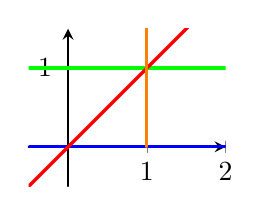
\begin{tikzpicture}[samples=100, line cap=round,line join=round,>=triangle 45,x=1cm,y=1cm]
			\begin{axis}[
				x=1cm,y=1cm,
				axis lines=middle,
				xmin=-0.5,
				xmax=2,
				ymin=-0.5,
				ymax=1.5,
				xtick={-10,-9,...,10},
				ytick={-2,...,10},]
				\addplot[very thick, blue] {0};
				\addplot[very thick, green] {1};
				\addplot[very thick, red] {x};
				\addplot[orange, very thick] coordinates {(1,2) (1,0)};
			\end{axis}
		\end{tikzpicture}
	\end{figure}
	\[\begin{split}
		\int\limits_0^1\int\limits_y^1 \frac{\sin x}{x}\dd{x}\dd{y}&=\int\limits_0^1\int\limits_0^x \frac{\sin x}{x}\dd{y}\dd{x}\\
		&=1-\cos 1
	\end{split}\]
\end{explanation}
\begin{eg}
	Evaluate
	\[\int\limits_0^\infty \frac{e^{-ax}-e^{-bx}}{x}\dd{x}\]
\end{eg}
\begin{explanation}
	We can convert the integral into the following,
	\[\begin{split}
		\int\limits_0^\infty \frac{e^{-ax}-e^{-bx}}{x}\dd{x}&=\int\limits_0^\infty \int\limits_a^b e^{-yx}\dd{y}\dd{x}\\
		&=\int\limits_a^b\int\limits_0^\infty e^{-yx}\dd{x}\dd{y}\\
		=\ln\frac{b}{a}
	\end{split}\]
\end{explanation}
\section{Change of Variables}
Consider the integral,
\[\iint f(x,y)\dd{x}\dd{y}\]
Now, if $x=p_1(u,v)$ and $y=p_2(u,v)$, then the integral can be expressed as,
\[\iint g(u,v)\mathbb{J}(u,v) \quad \left( \mathbb{J}(u,v)=\frac{\partial(x,y)}{\partial(u,v)} \right)\]
\begin{theorem}[Gaussian Integral]
	The function $f(x)=e^{-x^2}$ is called the Gaussian function. It does not have an elementary indefinite integral. But the total area under the area can be calculated.
	\[\int\limits_0^\infty e^{-x^2}\dd{x}\]
\end{theorem}
\begin{proof}
	Let,
	\[\begin{split}
		I&=\int\limits_0^\infty e^{-x^2}\dd{x}\\
		I&=\int\limits_0^\infty e^{-y^2}\dd{y}\\
		\implies I^2&=\left(\int\limits_0^\infty e^{-x^2}\dd{x}\right)\left(\int\limits_0^\infty e^{-y^2}\dd{y}\right)
	\end{split}\]
	Here, since the variables are independent, then the integral can be resolved into a double integral,
	\[\begin{split}
		I^2&=\int\limits_0^\infty\int\limits_0^\infty e^{-(x^2+y^2)}\dd{x}\dd{y}
	\end{split}\]
	Now, changing into polar coordinates, i.e.,
	\[x=r\cos\theta \land y=r\sin\theta \land \mathbb{J}(u,v)=r\]
	The limits are now changed to,
	\[r\in(0,\infty) \land \theta in \left(0,\frac{\pi}{2}\right)\]
	\[\begin{split}
		I^2&=\int\limits_0^\frac{\pi}{2}\int\limits_0^\infty e^{-r^2}\cdot r\dd{r}\dd{\theta}\\
		I^2&=\frac{\pi}{4}\\
		\therefore I&=\frac{\sqrt{\pi}}{2}
	\end{split}\]
\end{proof}
\subsection{Integrals using Polar Coordinate Systems}
\subsubsection{Cardioid}
	\begin{figure}[H]
		\centering
	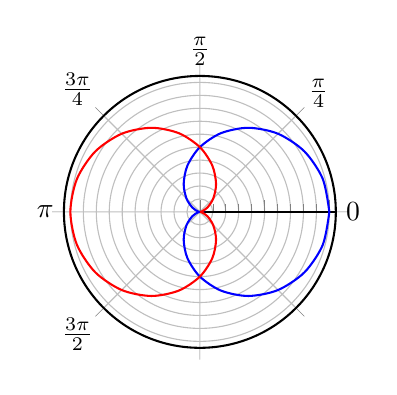
\begin{tikzpicture}
		\begin{polaraxis}[
			width=0.7\textwidth, % Adjust the width of the plot
			grid=both, % Show grid lines
			minor y tick num=4, % Number of minor ticks on y-axis
			minor x tick num=1, % Number of minor ticks on x-axis
			xtick={0,0,45,90,135,180,225,270,315}, % Define x-axis tick marks in degrees
			xticklabels={,0,$\frac{\pi}{4}$,$\frac{\pi}{2}$,$\frac{3\pi}{4}$,$\pi$,$\frac{3\pi}2$},
			ytick={0,1,2},
			yticklabels= \empty,
			ymax=2.1, % Set the maximum value of r
			smooth, % Smooth out the curve
			scale=0.5,
			]
			
			% Plot a cardioid with a=1
			\addplot[mark=none,blue,domain=0:360] {1 + cos(x)};
			\addplot[mark=none,red,domain=0:360] {1 - cos(x)};
		\end{polaraxis}
	\end{tikzpicture}
	\caption*{\color{blue} $r=1+\cos\theta$ \color{black}and \color{red} $r=1-\cos\theta$}
\end{figure}
\begin{eg}
	Evaluate $\iint 3y\dd{A}$ above the x-axis and below the cardioid $r=1-\cos\theta$.
\end{eg}
\begin{explanation}
\begin{figure}[H]
	\centering
		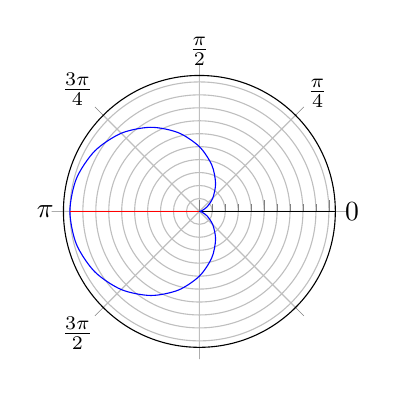
\begin{tikzpicture}
		\begin{polaraxis}[
			width=0.7\textwidth, % Adjust the width of the plot
			grid=both, % Show grid lines
			minor y tick num=4, % Number of minor ticks on y-axis
			minor x tick num=1, % Number of minor ticks on x-axis
			xtick={0,0,45,90,135,180,225,270,315}, % Define x-axis tick marks in degrees
			xticklabels={,0,$\frac{\pi}{4}$,$\frac{\pi}{2}$,$\frac{3\pi}{4}$,$\pi$,$\frac{3\pi}2$},
			ytick={0,1,2},
			yticklabels= \empty,
			ymax=2.1, % Set the maximum value of r
			smooth, % Smooth out the curve
			scale=0.5,
			]
			
			% Plot a cardioid with a=1
			\addplot[mark=none,blue,domain=0:360, name path=G] {1 - cos(x)};
			\addplot[red, name path=xAxis] coordinates {(0,0) (180,2)};
			\addplot[fill=black, opacity=0.2] fill between [of=G and xAxis, soft clip={domain=-179:180}];
		\end{polaraxis}
	\end{tikzpicture}
\end{figure}
Here, 
\[r\in (0,1-\cos\theta) \land \theta\in(0,\pi)\]
Thus, the integral can be written as,
\[\begin{split}
	I&=\int\limits_0^\pi\int\limits_0^{1-\cos\theta}3r\sin\theta\cdot r\dd{r}\dd{\theta}\\
	&=4
\end{split}\]
\end{explanation}
\begin{eg}
	Find the area common the cardioids, $r=1-\cos\theta$ and $r=1+\cos\theta$.
\end{eg}
\begin{explanation}
	\begin{figure}[H]
		\centering
		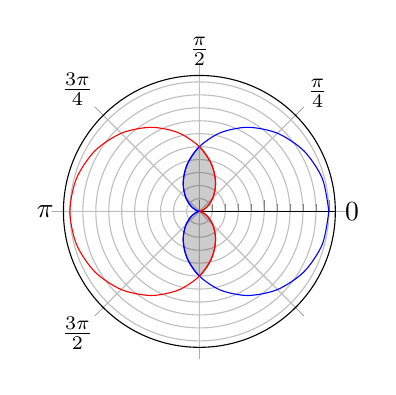
\begin{tikzpicture}
			\begin{polaraxis}[
				width=0.7\textwidth, % Adjust the width of the plot
				grid=both, % Show grid lines
				minor y tick num=4, % Number of minor ticks on y-axis
				minor x tick num=1, % Number of minor ticks on x-axis
				xtick={0,0,45,90,135,180,225,270,315}, % Define x-axis tick marks in degrees
				xticklabels={,0,$\frac{\pi}{4}$,$\frac{\pi}{2}$,$\frac{3\pi}{4}$,$\pi$,$\frac{3\pi}2$},
				ytick={0,1,2},
				yticklabels= \empty,
				ymax=2.1, % Set the maximum value of r
				smooth, % Smooth out the curve
				scale=0.5,
				]
				
				% Plot a cardioid with a=1

				\addplot[mark=none,blue,domain=90:180, name path =A1] {1 + cos(x)};
				\addplot[mark=none,blue,domain=180:270, name path =A2] {1 + cos(x)};
				\addplot[mark=none,red,domain=0:90, name path=B1] {1 - cos(x)};
				\addplot[mark=none,red,domain=270:360, name path=B2] {1 - cos(x)};
				\addplot[fill=black, opacity=0.2] fill between [of=A1 and B1, soft clip];
				\addplot[fill=black, opacity=0.2] fill between [of=A2 and B2, soft clip];
				\addplot[mark=none,blue,domain=0:360] {1 + cos(x)};
				\addplot[mark=none,red,domain=0:360] {1 - cos(x)};
			\end{polaraxis}
		\end{tikzpicture}
	\end{figure}
	By symmetry,
	\[\begin{split}
		I&=4\int\limits_0^\frac{\pi}{2}\int\limits_0^{1-\cos\theta}r\dd{r}\dd{\theta}\\
		&=\frac{3\pi}{4}-4
	\end{split}\]
\end{explanation}
\section{Triple Integrals}
\begin{theorem}
	The conversion of Cartesian coordinates to spherical coordinates can be done by,
	\[\begin{split}
		x&=r\cos\theta\sin\phi\\
		y&=r\sin\theta\sin\phi\\
		z&=r\cos\phi
	\end{split}\]
	And the Jacobian is given by,
	\[\mathbb{J}(r\theta,\phi)=r^2\sin\phi\]
	And the angles lie between,
	\[\theta \in [0,2\pi] \land \phi\in[0,\pi] \]
\end{theorem}
\begin{eg}
	Evaluate $\iiint\limits_D x^2+y^2+z^2\dd{x}\dd{y}\dd{z}$ where $D=\{(x,y,z)\in\mathbb{R}^3 : x^2+y^2+z^2\leq 1\}$.
\end{eg}
\begin{explanation}
	Converting to polar coordinates,
	\[r\in[0,1]\land \theta\in[0,2\pi]\land \phi\in[0,\pi]\]
	We get,
	\[\begin{split}
		I&=\int\limits_0^\phi\int\limits_0^{2\pi}\int\limits_0^1 r^2\cdot r^2\sin\phi\dd{r}\dd{\theta}\dd{\phi}\\
		&=\left(\int\limits_0^1r^4\dd{r}\right)\left(\int\limits_0^{2\pi}\dd{\theta}\right)\left(\int\limits_0^\pi\sin\phi\dd{\phi}\right)\\
		&=\frac{4\pi}{5}
	\end{split}\]
\end{explanation}
\begin{eg}[Not sure]
	Evaluate the integral $\iint\limits_D xy\sqrt{1-x-y}\dd{x}\dd{y}$, where $D$ is the region bounded by $x=0$, $y=0$ and $x+y=1$ using the transform $x+y=u$ and $xy=v$.
\end{eg}
\begin{explanation}
	Using the transformation of variables, we get,
	\[u(1-v)=0\land uv=0\land u=1\]
	\[u\in[0,1]\land v\in[0,1]\]
	The Jacobian is,
	\[\mathbb{J}(u,v)=u\]
	Thus, the integral is,
	\[\begin{split}
		I&=\int\limits_0^1\int\limits_0^1v\sqrt{1-u}\cdot u\dd{u}\dd{v}\\
		&=\frac{2}{15}
	\end{split}\]
\end{explanation}
\begin{eg}
	Find the volume of the solid surrounded by the surface $\left(\frac{x}{a}\right)^\frac{2}{3}+\left(\frac{y}{b}\right)^\frac{2}{3}+\left(\frac{z}{c}\right)^\frac{2}{3}=1$.
\end{eg}
\begin{explanation}
	First, choose,
	\[\left(\frac{x}{a}\right)^\frac{2}{3}=u\land \left(\frac{y}{b}\right)^\frac{2}{3}=v\land \left(\frac{z}{c}\right)^\frac{2}{3}=w\]
	Thus, the curve is,
	\[S:u^2+v^2+w^2=1\quad(\text{A unit sphere})\]
	The Jacobian is,
	\[\mathbb{J}(u,v,w)=27abc\cdot u^2v^2w^2\]
	The integral now is,
	\[I=\iiint\limits_S 27abc\cdot u^2v^2w^2 \dd{V}\]
	Now, converting to spherical coordinates,
	\[u=r\cos\theta\sin\phi\land v=r\sin\theta\sin\phi\land w=r\cos\phi\]
	The limits are
	\[r\in[0,1]\land \theta\in[0,2\pi]\land \phi\in[0,\pi]\]
	Thus, the final integral is,
	\[\begin{split}
		I&=27abc\int\limits_0^{2\pi}\int\limits_0^\pi\int\limits_0^1 (r^3\sin^2\phi\cos\phi\sin\theta\cos\theta)^2\cdot r^2\sin\phi\dd{r}\dd{\phi}\dd{\theta}]\\
		&=27abc\left( \int\limits_0^1 r^8\dd{r} \right)\left(\int\limits_0^\pi \sin^5\phi\cos^2\phi\right)\left(\int\limits_0^{2\pi} \sin^2\theta\cos^2\theta\dd{\theta}\right)\\
		&=\frac{4\pi abc}{35}
	\end{split}\]
\end{explanation}
\section{Beta Function}
The function is defined as,
\[\beta(m,n)=\int\limits_0^1x^{m-1}(1-x)^{n-1}\dd{x}\quad m,n\geq 1\]
\begin{theorem}[Symmetry]
	\[\beta(m,n)=\beta(n,m)\]
\end{theorem}
\begin{theorem}
	\[\beta(m,n)=2\int\limits_0^\frac{\pi}{2}\sin^{2m-1}\theta \cos^{2n-1}\theta\dd{\theta}\]
\end{theorem}
\section{Gamma Function}
This is an extension to the factorial,
\[\Gamma(n)=\int\limits_0^\infty e^{-x}x^{n-1}\dd{x}=(n-1)!\]
\section{Tutorial-6}
\subsection{Evaluate the double integrals}
\begin{asign}
	$\iint\limits_Rx^2\dd{A}$, where $R$ is the region bounded by $y=x^2$, $y=x+2$.
\end{asign}
\begin{anse}
	The region described is,
	\[x\in[-1,2] \land x^2\leq y\leq x+2\]
	Thus, the integral is,
	\[\begin{split}
		I&=\int\limits_{-1}^2\int\limits_{x^2}^{x+2}x^2\dd{y}\dd{x}\\
		&=\frac{163}{60}
	\end{split}\]
\end{anse}
\begin{asign}
	$\iint\limits_R (x^2+y^2)\dd{A}$, where $R:0\leq y\leq \sqrt{1-x^2}, \; 0\leq x\leq 1$.
\end{asign}
\begin{anse}
	Clearly,
	\[\begin{split}
		I&=\int\limits_0^1\int\limits_{0}^{\sqrt{1-x^2}}x^2+y^2\dd{y}\dd{x}\\
		&=\frac{\pi}{8}
	\end{split}\]
\end{anse}
\begin{asign}
	$\iint\limits_R a^2-x^2-y^2\dd{A}$, where $R$ is the region $x^2+y^2\leq a^2$.
\end{asign}
\begin{anse}
	The region described is,
	\[x\in[-1,1] \land -\sqrt{a^2-x^2}\leq y\leq \sqrt{a^2-x^2} \quad(\because \text{ Upper and lower parts of the disc})\]
	Thus,
	\[\begin{split}
		I&=\int\limits_{-1}^1\int\limits_{-\sqrt{a^2-x^2}}^{\sqrt{a^2-x^2}}a^2-x^2-y^2\dd{y}\dd{x}\\
		&=\text{Something}
	\end{split}\]
	The better way is to change into polar coordinates, since the region described is a complete circle,
	\[r\in[0,a] \land \theta\in[0,2\pi]\]
	Thus, the integral is,
	\[\begin{split}
		I&=\int\limits_0^a\int\limits_0^{2\pi}(a^2-r^2)\cdot r\dd{\theta}\dd{r}\\
		&=\left(\int\limits_0^aa^2r-r^3\dd{r}\right)\left(\int\limits_0^{2\pi}\dd{\theta}\right)\\
		&=\frac{\pi a^4}{2}
	\end{split}\]
\end{anse}
\begin{asign}
	$\iint\limits_R xy\dd{x}\dd{y}$, where $R$ is the region bounded by $x$-axis, ordinate $x=2a$ and the curve $x^2=4ay$.
\end{asign}
\begin{anse}
	The region described is,
	\[y\in[0,a]\land 2\sqrt{ay}\leq x\leq 2a\]
	Thus, the integral is,
	\[\begin{split}
		I&=\int\limits_0^a\int\limits_{2\sqrt{ay}}^{2a}xy\dd{x}\dd{y}\\
		&=\frac{a^4}{3}
	\end{split}\]
\end{anse}
\begin{asign}
	$\iint\limits_0^R x^2\dd{x\dd{y}}$, where $R$ is the region in the first quadrant bounded by the lines $x=y$, $y=0$, $x=8$ and the curve $xy=16$.
\end{asign}
\begin{anse}
	The region can be described in the following way,
	\[\left( x\in[0,4] \land 0\leq y\leq x \right) \land \left( x\in[4,8]\land 0\leq y \leq \frac{16}{x}\right)\]
	\begin{figure}[H]
		\centering
		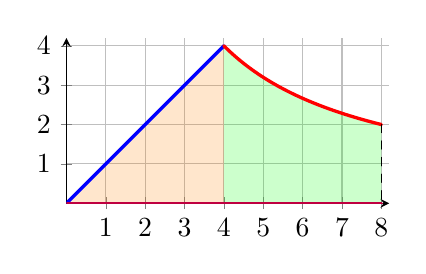
\begin{tikzpicture}[samples=150, line cap=round,line join=round,>=triangle 45,x=1cm,y=1cm]
			\begin{axis}[
				x=1cm,y=1cm,
				axis lines=middle,
				ymajorgrids=true,
				xmajorgrids=true,
				xmin=-0,
				xmax=8.2,
				ymin=-0,
				ymax=4.2,
				xtick={-7,-6,...,10},
				ytick={-4,-3,...,10},
				scale=0.5,]
				\addplot[very thick, blue, name path=line, domain=0:4] plot(\x, \x);
				\addplot[very thick, red, name path=hyper, domain=4:8] {16/x};
				\addplot[very thick, purple, name path=xAxis, domain=0:8] {0};
				\draw[dashed] (8,-2) -- (8,2);
				\addplot[fill=orange, opacity=0.2] fill between[of=xAxis and line, soft clip={domain=0:4}];
				\addplot[fill=green, opacity=0.2] fill between[of=xAxis and hyper, soft clip={domain=4:8}];
			\end{axis}
		\end{tikzpicture}
	\end{figure}
	Thus, the integral is,
	\[\begin{split}
		I&=\int\limits_0^4\int\limits_0^xx^2\dd{y}\dd{x}+\int\limits_4^8\int\limits_0^\frac{16}{x}x^2\dd{y}\dd{x}\\
		&=448
	\end{split}\]
\end{anse}
\begin{asign}
	$\iint r^3\dd{r}\dd{\theta}$, over the area included between $r=2\sin\theta$ and $r=4\sin\theta$.
\end{asign}
\begin{anse}
	Clearly,
	\begin{figure}[H]
		\centering
		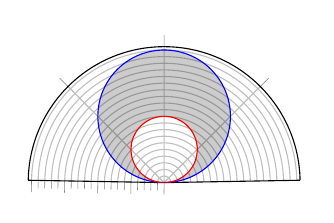
\begin{tikzpicture}
			\begin{polaraxis}[
				width=0.7\textwidth, % Adjust the width of the plot
				grid=both, % Show grid lines
				minor y tick num=4, % Number of minor ticks on y-axis
				minor x tick num=1, % Number of minor ticks on x-axis
				xtick={0,0,45,90,135,180,225,270,315}, % Define x-axis tick marks in degrees
				xticklabels=\empty,
				xmin=1,
				xmax=179,
				ytick={0,1,2,3,4},
				yticklabels= \empty,
				ymax=4.1, % Set the maximum value of r
				smooth, % Smooth out the curve
				scale=0.5,
				]
				
				\addplot[blue, name path=upper, domain=0:360, samples=100] {4*sin(x)};
				\addplot[red, name path=lower, domain=0:360, samples=100] {2*sin(x)};
				\addplot[fill=black, opacity=0.2] fill between[of=upper and lower, soft clip={domain=-179:179}];
			\end{polaraxis}
		\end{tikzpicture}
	\end{figure}
	\[\theta\in [0,\pi]\land 2\sin\theta \leq r\leq 4\sin\theta\]
	Thus, the integral is,
	\[\begin{split}
		I&=\int\limits_0^\pi\int\limits_{2\sin\theta}^{4\sin\theta}r^3\dd{r}\dd{\theta}\\
		&=\frac{90\pi}{4}
	\end{split}\]
\end{anse}
\subsection{Evaluate the following integrals by changing the order of integration if needed}
\begin{asign}
	\[\int\limits_0^3\int\limits_{-y}^yx^2+y^2\dd{x}\dd{y}\]
\end{asign}
\begin{anse}
	Here the limits are,
	\[y\in[0,3]\land -y\leq x\leq y\]
	These are equivalent to,
	\[\left(x\in[-3,0]\land -x\leq y\leq 3\right)\land \left(x\in[0,3]\land x\leq y\leq 3\right)\]
	Thus, the integral is,
	\[\begin{split}
		I&=\int\limits_{-3}^0\int\limits_{-x}^3x^2+y^2\dd{y}\dd{x}+\int\limits_{0}^3\int\limits_{x}^3x^2+y^2\dd{y}\dd{x}\\
		&=\frac{54}{3}
	\end{split}\]
\end{anse}
\begin{asign}
	\[\int\limits_0^1\int\limits_2^{4-2x}\dd{y}\dd{x}\]
\end{asign}
\begin{anse}
	Here the limits are,
	\[x\in[0,1]\land 2\leq y\leq 4-2x\]
	These are equivalent to,
	\[y\in[2,4]\land 0\leq x\leq \frac{4-y}{2}\]
	Thus, the integral is,
	\[\begin{split}
		I&=\int\limits_2^4\int\limits_0^{\frac{4-y}{2}}\dd{x}\dd{y}\\
		&=1
	\end{split}\]
\end{anse}
\begin{asign}
	\[\int\limits_0^\frac{3}{2}\int\limits_0^{9-4x^2}16x\dd{y}\dd{x}\]
\end{asign}
\begin{anse}
	Here the limits are,
	\[x\in[0,\frac{3}{2}]\land 0\leq y\leq 9-4x^2\]
	These are equivalent to,
	\[y\in[0,9]\land 0\leq x\leq \frac{\sqrt{9-y}}{2}\]
	Thus, the integral is,
	\[\begin{split}
		I&=\int\limits_0^9\int\limits_0^{\frac{\sqrt{9-y}}{2}}16x\dd{x}\dd{y}\\
		&=81
	\end{split}\]
\end{anse}
\begin{asign}
	\[\int\limits_0^2\int\limits_0^{4-x^2}\frac{xe^{2y}}{4-y}\dd{y}\dd{x}\]
\end{asign}
\begin{anse}
	Here the limits are,
	\[x\in[0,2]\land 0\leq y\leq 4-x^2\]
	These are equivalent to,
	\[y\in[0,4]\land 0\leq x\leq \sqrt{4-y}\]
	Thus, the integral is,
	\[\begin{split}
		I&=\int\limits_0^4\int\limits_0^{\sqrt{4-y}}\frac{xe^{2y}}{4-y}\dd{x}\dd{y}\\
		&=\frac{e^8}{4}-\frac{1}{4}
	\end{split}\]
\end{anse}
\begin{asign}
	\[\int\limits_{-a}^a\int\limits_0^{\sqrt{a^2-y^2}}f(x,y)\dd{x}\dd{y}\]
\end{asign}
\begin{anse}
	Here the limits are,
	\[y\in[-a,a]\land 0\leq x\leq \sqrt{a^2-y^2}\]
	These are equivalent to,
	\[x\in[0,a]\land -\sqrt{a^2-x^2}\leq y\leq \sqrt{a^2-x^2}\]
	Thus, the integral is,
	\[I=\int\limits_0^a\int\limits_{-\sqrt{a^2-x^2}}^{\sqrt{a^2-x^2}}f(x,y)\dd{y}\dd{x}\]
\end{anse}
\begin{asign}
	\[\int\limits_0^1\int\limits_{e^x}^e\frac{1}{\ln y}\dd{y}\dd{x}\]
\end{asign}
\begin{anse}
	Here the limits are,
	\[x\in[0,1]\land e^x\leq y\leq e\]
	These are equivalent to,
	\[y\in[1,e]\land 0\leq x\leq \ln y\]
	Thus, the integral is,
	\[\begin{split}
		I&=\int\limits_1^e\int\limits_0^{\ln y}\frac{1}{\ln y}\dd{x}\dd{y}\\
		&=e-1
	\end{split}\]
\end{anse}
\begin{asign}
	By changing the order of integration of $\int\limits_0^\infty\int\limits_0^\infty e^{-xy}\sin px\dd{x}\dd{y}$, show that $\int\limits_0^\infty \frac{\sin px}{x}=\frac{\pi}{2}$.
\end{asign}
\begin{anse}
	Let,
	\[I=\int\limits_0^\infty\int\limits_0^\infty e^{-xy}\sin px\dd{x}\dd{y}\]
	Changing the order of integration we get,
	\[\begin{split}
		I&=\int\limits_0^\infty\int\limits_0^\infty e^{-xy}\sin px\dd{y}\dd{x}\\
		&=\int\limits_0^\infty \sin px \frac{-1}{x}\eval{e^{-xy}}_{0}^{\infty}\dd{x}\\
		\therefore I&=\int\limits_0^\infty \frac{\sin px}{x}\dd{x}
	\end{split}\]
	Integrating the original integral,
	\[\begin{split}
		I&=\int\limits_0^\infty \eval{\frac{e^{-yx}}{y^2-p^2}(-y\sin px-p\cos px)}_{0}^{\infty} \dd{y}\\
		\therefore I&=\frac{\pi}{2}
	\end{split}\]
	Thus, also,
	\[\int\limits_0^\infty \frac{\sin px}{x}=\frac{\pi}{2}\]
\end{anse}
\subsection{Find the volume of the following}
\begin{asign}
	Region bounded above by the cylinder $z=x^2$ and below by the region enclosed by the parabola $y=2-x^2$ and the line $y=x$ in the $xy$ plane.
\end{asign}
\begin{anse}
	Clearly the integral set-up is,
	\[I=\iint\limits_\Omega x^2\dd{A}\]
	The region $\Omega$ can be described as,
	\[x\in[-2,1]\land x\leq y\leq 2-x^2\]
	Integrating,
	\[\begin{split}
		I&=\int\limits_0^1\int\limits_x^{2-x^2} x^2\dd{y}\dd{x}\\
		&=\frac{63}{20}
	\end{split}\]
\end{anse}
\subsection{Use the given transformations to transform the integrals and evaluate them}
\begin{asign}
	$u=3x+2y$, $v=x+4y$ and $I=\iint\limits_R (3x^2+14xy+8y^2)\dd{A}$ where $R$ is the region in the first quadrant bounded by the lines $y+\frac{3x}{2}=1$, $y+\frac{3x}{2}=3$, $y+\frac{x}{4}=0$ and $y+\frac{x}{4}=1$.
\end{asign}
\begin{anse}
	The area bound is a parallelogram,
	\[x=\frac{4u-2v}{10}\land y=\frac{3v-u}{10}\]
	The limits are,
	\[u\in[2,6]\land v\in[0.4]\]
	The Jacobian is,
	\[\mathbb{J}(u,v)=\frac{\partial(x,y)}{\partial(u,v)}=\begin{vmatrix}
		\frac{2}{5} & \frac{-1}{5}\\
		\frac{-1}{10} & \frac{3}{10}
	\end{vmatrix}=\frac{1}{10}\]
	Thus, the integral is,
	\[\begin{split}
		I&=\int\limits_2^6\int\limits_0^4 uv\cdot\frac{1}{10}\dd{v}\dd{u}\\
		&=12.8
	\end{split}\]
\end{anse}
\begin{asign}
	$u=x+2y$, $v=x-y$ and $I=\int\limits_0^\frac{2}{3}\int\limits_y^{2-2y}(x+2y)e^{y-x}\dd{A}$.
\end{asign}
\begin{anse}
	The limits are,
	\[u\in[0,2]\land v\in[0,u]\]
	The Jacobian is,
	\[\mathbb{J}(u,v)=\frac{1}{J(x,y)}=\frac{1}{\begin{vmatrix}
			1 & 2\\
			1 & -1
	\end{vmatrix}}=\frac{-1}{3}\implies |\mathbb{J}(u,v)|=\frac{1}{3}\]
	Thus, the integral is,
	\[\begin{split}
		I&=\int\limits_0^2\int\limits_0^u ue^{-v}\cdot \frac{1}{3}\dd{v}\dd{u}\\
		&=\frac{3e^{-2}+1}{3}
	\end{split}\]
\end{anse}
\begin{asign}
	$u=xy$, $v=x^2-y^2$ and $I=\iint\limits_R(x^2+y^2)\dd{A}$, where $R$ is the region bounded by $xy=1$, $xy=2$, $x^2-y^2=1$ and $x^2-y^2=2$.
\end{asign}
\begin{anse}
	The limits are,
	\[u\in[1,2]\land v\in[1,2]\]
	The Jacobian is,
	\[\mathbb{J}(u,v)=\frac{1}{\mathbb{J}(x,y)}=\frac{1}{\begin{vmatrix}
			y& x\\
			2x & -2y
	\end{vmatrix}}=\frac{-1}{2(x^2+y^2)} \implies |\mathbb{J}(u,v)|=\frac{1}{2(x^2+y^2)}\]
	The integral is,
	\[\begin{split}
		I&=\int_1^2\int_1^2 (x^2+y^2)\cdot \frac{1}{2(x^2+y^2)} \dd{v}\dd{u}\\
		&=\frac{1}{2}
	\end{split}\]
\end{anse}
\begin{asign}
	$x=au$, $y=bv$, $z=cw$, and $I=\iiint_D \dd{V}$ where $D$ is the ellipsoid : $\frac{x^2}{a^2}+\frac{y^2}{b^2}+\frac{z^2}{c^2}=1$.
\end{asign}
\begin{anse}
	The Jacobian is,
	\[\mathbb{J}(u,v,w)=\frac{1}{\begin{vmatrix}
			a & 0 & 0\\
			0 & b & 0\\
			0 & 0 & c
	\end{vmatrix}}=abc \]
	The ellipsoid is converted to,
	\[S: u^2+v^2+w^2=1\]
	Which is a unit sphere.
	The integral is,
	\[\begin{split}
		I&=\iiint_{S}abc\dd{V}\\
		&=\frac{4abc}{3}\pi
	\end{split}\]
\end{anse}
\begin{asign}
	$u=x$, $v=xy$, $w=3z$ and $I=\iiint_D x^2y+3xyz\dd{V}$ where $D=\{(x,y,z)\in\mathbb{R}^3 : 1\leq x \leq 2, 0\leq xy\leq 2, 0\leq z\leq 1 \}$.
\end{asign}
\begin{anse}
	The limits are,
	\[u\in[1,2]\land v\in[0,2]\land w\in[0,3]\]
	The Jacobian is,
	\[\mathbb{J}(u,v,w)=\frac{1}{3u}\]
	Thus, the integral is,
	\[\begin{split}
		I&=\int\limits_0^3\int\limits_0^2\int\limits_1^2v+\frac{vw}{u}\dd{u}\dd{v}\dd{w}\\
		&=2+3\ln 2
	\end{split}\]
\end{anse}
\begin{asign}
	Using appropriate transformation evaluate $\iint_R\dd{A}$, where $R$ is the parallelogram with vertices $(1,0)$, $(3,1)$, $(2,2)$ and $(0,1)$.
\end{asign}
\begin{anse}
	The equations for the parallel lines are,
	\[x+y=1\land x+y=4 \land x-2y=1\land x-2y=-1\]
	Thus, consider the transformation,
	\[u=x+y\land v=x-2y\]
	Thus, the limits are,
	\[u\in[1,4]\land v\in [-1,1]\]
	The Jacobian is,
	\[\mathbb{J}(u,v)=\frac{1}{\mathbb{J}(x,y)}=\frac{-1}{3}\implies |\mathbb{J}|=\frac{1}{3}\]
	Thus, the integral is,
	\[\begin{split}
		I&=\int\limits_1^4\int\limits_{-1}^1\frac{1}{3}\dd{v}\dd{u}\\
		&=2
	\end{split}\]
\end{anse}
\subsection{Evaluate the following volume integrals}
\begin{asign}
	$\iiint\limits_D (z^2x^2+z^2y^2)\dd{V}$, where $D=\{(x,y,z)\in\mathbb{R}^3:x^2+y^2\leq 1, -1\leq z\leq 1\}$.
\end{asign}
\begin{anse}
	Converting to cylindrical coordinates,
	\[r\in[0,1]\land \theta\in[0,2\pi]\land z\in[-1,1]\]
	Thus, the integral is,
	\[\begin{split}
		I&=\int\limits_{-1}^1\int\limits_0^{2\pi}\int\limits_0^1r^2z^2\cdot r\dd{r}\dd{\theta}\dd{z}\\
		&=\frac{\pi}{3}
	\end{split}\]
\end{anse}
\begin{asign}
	$\iiint\limits_D xyz\dd{V}$, where $D=\{(x,y,z)\in\mathbb{R}^3:x^2+y^2\leq1, 0\leq z\leq x^2+y^2\}$.
\end{asign}
\begin{anse}
	Converting to cylindrical coordinates,
	\[r\in[0,1]\land \theta\in[0,2\pi]\land z\in[0,r^2]\]
	Thus, the integral is,
	\[\begin{split}
		I&=\int\limits_0^{2\pi}\int\limits_0^1\int\limits_0^{r^2}zr^2\sin\theta\cos\theta\cdot r\dd{z}\dd{r}\dd{\theta}\\
		&=0
	\end{split}\]
\end{anse}
\begin{asign}
	$\iiint\limits_D e^{(x^2+y^2+z^2)^\frac{3}{2}}\dd{V}$, where $D=\{(x,y,z)\in\mathbb{R}^3:x^2+y^2+z^2\leq 1\}$.
\end{asign}
\begin{anse}
	Converting to spherical coordinates,
	\[r\in[0,1]\land \theta\in[0,2\pi]\land \phi\in[0,\pi]\]
	Thus, the integral is,
	\[\begin{split}
		I&=\int\limits_0^{2\pi}\int\limits_0^{\pi}\int\limits_0^1e^{r^3}\cdot r^2\sin\phi \dd{r}\dd{\phi}\dd{\theta}\\
		&=\frac{4\pi(e-1)}{3}
	\end{split}\]
\end{anse}
\subsection{Using Beta and Gamma functions, evaluate the following}
\begin{asign}
	\[\int\limits_0^\infty e^{-x^2}\dd{x}\]
\end{asign}
\begin{asign}
	\[\int\limits_0^\frac{\pi}{2}\sqrt{\tan x}\dd{x}\]
\end{asign}
\begin{asign}
	\[\int\limits_0^1x^m\left(\ln\frac{1}{x}\right)^n\dd{x}\]
\end{asign}
\begin{asign}
	\[\int\limits_0^\frac{\pi}{2}\sin^4\theta\cos^6\theta\dd{\theta}\]
\end{asign}
\begin{asign}
	\[\int\limits_0^\infty\frac{x^c}{c^x}\dd{x}\]
\end{asign}
\begin{asign}
	\[\int\limits_0^\infty a^{-bx^2}\dd{x}\]
\end{asign}
\begin{asign}
	\[\int_0^1x^5\left(\ln\frac{1}{x}\right)^3\dd{x}\]
\end{asign}
\begin{asign}
	Express $\int_0^1x^m(1-x^p)^n\dd{x}$ in terms of Beta function and hence evaluate the integral,
	\[\int\limits_0^1 x^\frac{3}{2}(1-\sqrt{x})^{\sqrt{12}} \dd{x}\]
\end{asign}
\begin{asign}
	Show that,
	\[\beta(p,q)=\int\limits_0^\infty\frac{y^{q-1}}{(1+y)^{p+q}}\dd{y}=\int\limits_0^1\frac{x^{p-1}+y^{q-1}}{(1+x)^{p+q}}\]
\end{asign}




















\end{document}